\documentclass[review]{siamart1116}

\usepackage{lipsum}
\usepackage{amsfonts}
\usepackage{graphicx}
\usepackage{epstopdf}
\usepackage{algorithmic}
\ifpdf
  \DeclareGraphicsExtensions{.eps,.pdf,.png,.jpg}
\else
  \DeclareGraphicsExtensions{.eps}
\fi

\numberwithin{theorem}{section}

\newcommand{\TheTitle}{Certifying unstability of Switched Systems using Sum of Squares Programming}
\newcommand{\TheAuthors}{B. Legat, R. M. Jungers, and P. A. Parrilo}

\headers{\parbox{0.92\textwidth}{\TheTitle}}{\TheAuthors}

\title{{\TheTitle}\thanks{Submitted to the editors September 28, 2017.
A preliminary version of this work appeared in Proceedings of Hybrid Systems: Computation and Control, 2016 \cite{legat2016generating}.
}}

\author{
  Beno\^{i}t Legat%
  \thanks{ICTEAM, Universit\'e catholique de Louvain, 4 Av. G. Lema\^itre, 1348 Louvain-la-Neuve, Belgium
    (\email{benoit.legat@uclouvain.be}).}
  \and
  Pablo A. Parrilo%
  \thanks{Laboratory for Information and Decision Systems, Massachusetts Institute of Technology, 77 Massachusetts Avenue, Cambridge MA 02139, USA
    (\email{parrilo@mit.edu}).}
  \and
  Rapha\"{e}l M. Jungers%
  \thanks{ICTEAM, Universit\'e catholique de Louvain, 4 Av. G. Lema\^itre, 1348 Louvain-la-Neuve, Belgium
    (\email{raphael.jungers@uclouvain.be}).}
}

\usepackage{amsopn}


\ifpdf
\hypersetup{
  pdftitle={\TheTitle},
  pdfauthor={\TheAuthors}
}
\fi

\usepackage{custom}
\usepackage{jsr}
\usepackage{tkz-graph}
../../latex/siamthm.tex

\begin{document}

\maketitle

\begin{abstract}
  ../../latex/absintro.tex

We show that the dual of this convex problem searches
for the \emph{occupations measures} of trajectories with high asymptotic growth
rate.
We both show how to generate a sequence of guaranteed high asymptotic growth rate and how to detect cases where we can provide lower bounds on the JSR.
We deduce from it a new guarantee for the upper bound provided by the sum of squares lyapunov program.
We end this paper with a method to reduce the computation of the JSR of
low rank matrices to the computation of the constrained JSR of matrices
of small dimension.

All results of this paper are presented for the general case of constrained switched systems,
that is, systems for which the switching signal is constrained by an automaton.

\end{abstract}

\begin{keywords}
  Joint spectral radius, Sum of squares programming,
  S\witch{} Systems, Path-complete Lyapunov functions
\end{keywords}

\begin{AMS}
  93D05, 93D20, 93D30
\end{AMS}

\section{Introduction}
In recent years, the study of the stability of hybrid systems
has been the subject of extensive research using methods based on classical ideas from Lyapunov theory
and modern mathematical optimization techniques.
Even for s\witch{} linear systems, arguably the simplest class of hybrid systems,
determining stability is undecidable and approximating the maximal asymptotic growth rate that a trajectory can have is NP-hard \cite{blondel2000boundedness}.
Despite these negative results, the vast range of applications has motivated a wealth of algorithms to approximate
this maximal asymptotic growth rate.


A s\witch{} linear system is characterized by a finite set of matrices $\A \eqdef \{A_1, A_2,\\\ldots, A_m\} \subset \mathbb{R}^{n \times n}$ and the iteration
\begin{equation}
  \label{eq:switchsys}
  x_k = A_{\sigma_k} x_{k-1}, \quad \sigma_k \in [m]
\end{equation}
where $[m]$ denotes the set $\{1, \ldots, m\}$.
The maximal asymptotic growth rate of this iteration is given by the \emph{joint spectral radius} (JSR).
The JSR $\jsr$ of a finite set of matrices $\A$
is defined as
\[ \jsr = \lim_{k \to \infty} \max_{\sigma \in [m]^k} \|A_{\sigma_k} \cdots A_{\sigma_2} A_{\sigma_1}\|^{1/k}. \]
This definition is independent of the norm used.


The JSR was introduced by Rota and Strang~\cite{rota1960note}
and has many other applications such as wavelets, the capacity of some particular codes, zero-order stability of ordinary differential equations, congestion control in computer networks, curve design and networked and delayed control systems; see \cite{jungers2009joint} for a survey on the JSR and its applications.
Many algorithms exist for estimating the JSR but not much is known on how to generate an infinite
sequence of matrices with an asymptotic growth rate close to the JSR.
However generating such sequence can be of particular interest, depending on the application,
such as exhibiting unstable trajectories for s\witch{} linear systems to prevent them from occuring~\cite{gomes2018minimally}.%
The currently known algorithms generate a sequence of matrices with high spectral radius
using methods detailed in \secref{lb}
and repeat this sequence infinitely \cite{gripenberg1996computing,guglielmi2008algorithm,guglielmi2013exact,jungers2014lifted}.

Approximating the JSR usually consists in certifying upper bounds $\gamub$ to the JSR by exhibiting a Lyapunov function or an invariant set for the matrices $A_i/\gamub$.
The search for such Lyapunov functions can naturally be written as a convex optimization program; see \progref{primalinf}.
Certifying lower bounds $\gamlb$ is currently either achieved using the guarantees we have on the accuracy of the upper bound on the JSR
or by exhibiting trajectories of asymptotic growth rate $\gamlb$.
In this paper, we introduce a new way to certify lower bounds by exhibiting nonnegative measures satisfying some invariance condition parametrized by the matrices $A_i/\gamlb$; see \eqref{eq:dualinf1}.
This invariance condition is linear on the measure hence the search of measures on the convex cone of nonnegative measures is a \emph{convex} program; see \progref{dualinf}.
It turns out that this program is the dual of \progref{primalinf}.

We revisit the sum-of-squares program proposed by Parrilo and Jadbabaie~\cite{parrilo2008approximation} and show that its dual formulation is the moment relaxation of the search of the measures satisfying the invariance condition.

Thanks to this duality, solving this pair of programs with a given candidate value $\gamma$
for the JSR either returns Lyapunov functions certifying that
$\jsr \leq \gamma$ or returns moments that form a solution of the moment relaxation; see \secref{moments}.
These moments are not necessarily the moments of measures satisfying the invariance conditions.
However, we give a rounding procedure to extract a (infinite) switching sequence from these moments
and provide a guarantee on the asymptotic growth rate of this sequence.
As a by-product of the rounding procedures, the spectral radius of a finite part of
this infinite sequence can be used to give lower bounds on the JSR.
In addition, we give a way to sometimes detect when the moments belongs to measures that satisfy the invariance conditions.
This happens when the measures are the convex combination of the occupation measures of several periodic trajectories.
Since the trajectories are periodic, the measures are atomic and we can recover them from moments of sufficiently high degree.
We show on numerical examples that these techniques work well in practice.


In some applications the values that $\sigma_k$ can take in \eqref{eq:switchsys} may depend on $\sigma_{k-1}, \sigma_{k-2},\\\ldots$.
These constraints are often conveniently represented using a \emph{finite automaton} and the JSR under such constraints
is called \emph{constrained joint spectral radius} (CJSR) \cite{dai2012gel}; an example of constrained s\witch{} system is given by \exemref{run1} and its automaton is illustrated by \figref{run}.


\begin{myexem}[Running example]%
  \label{exem:run1}
  We borrow the example of \cite[\Sect4]{philippe2016stability}.
  The set of matrices $\A$ is composed of the following four matrices
  \begin{align*}
    A_1 & = A+B
    \begin{pmatrix}
      k_1 & k_2
    \end{pmatrix},&
    A_2 & = A+B
    \begin{pmatrix}
      0 & k_2
    \end{pmatrix},\\
    A_3 & = A+B
    \begin{pmatrix}
      k_1 & 0
    \end{pmatrix},&
    A_4 & = A.
  \end{align*}
  where $k_1 = -0.49$, $k_2 = 0.27$,
  \[
    A =
    \begin{pmatrix}
      0.94 & 0.56\\
      0.14 & 0.46
    \end{pmatrix} \text{ and }
    B =
    \begin{pmatrix}
      0\\
      1
    \end{pmatrix}.
  \]

  The corresponding automaton is represented by Figure~\ref{fig:run}.

  \begin{figure}[!ht]
    \centering
    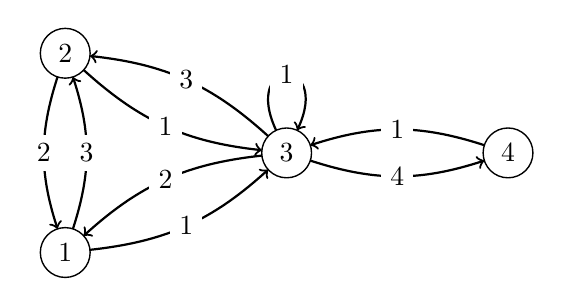
\begin{tikzpicture}[x=40,y=18]
       \Vertex{1}
       \NO[unit=4](1){2}
       \SOEA[unit=2](2){3}
       \EA[unit=2](3){4}
       \tikzset{EdgeStyle/.style = {->}}
       \tikzset{LoopStyle/.style = {->}}
       \tikzset{EdgeStyle/.append style = {bend right=18}}
       \Edge[label=1](1)(3)
       \Edge[label=3](1)(2)
       \Edge[label=2](2)(1)
       \Edge[label=1](2)(3)
       \Edge[label=2](3)(1)
       \Edge[label=3](3)(2)
       \Edge[label=4](3)(4)
       \draw[thick,->] (3) to [out=115,in=65,looseness=10] node [midway, fill=white] {1} (3);
       \Edge[label=1](4)(3)
     \end{tikzpicture}
     \caption{Automaton for the running example.
     The numbers on the \arcs{} are their respective labels.
     }
     \label{fig:run}
  \end{figure}
\end{myexem}


The automaton representing the constraints can be represented by a
strongly connected labelled directed graph $\G(\Nodes,\Arcs)$
of \nodes{} $\Nodes$ and \arcs{} $\Arcs$,
possibly with parallel \arcs{}.  The labels are elements of the set
$[m]$ and $\Arcs$ is a subset of $\Nodes \times \Nodes
\times [m]$.  We say that $(u,v,\sigma) \in \Arcs$ if
there is an \arc{} between node $u$ and node $v$ with label $\sigma$.
The iteration~\ref{eq:switchsys} is rewritten as follows to take the automaton into account:
\begin{equation}
  \label{eq:cswitchsys}
  x_k = A_{\sigma_k} x_{k-1}, \qquad (\sigma_1, \ldots, \sigma_k) \text{ are the respective labels of a path in }\G
  .
\end{equation}


The \emph{arbitrary switching} case~\eqref{eq:switchsys}
can be seen as the particular case when the automaton has only one node and $m$ self-loops with labels $1, \ldots, m$.
On the other side, any constrained switched system can be replaced by an arbitrary switching system with the same CJSR; see \lemref{koz}.

We also provide
a new estimate of the accuracy of the SOS-based approximation algorithm for the CJSR which is better
than the previously existing one for sufficiently large SOS degree.
The existing estimate only depends on the dimension of the matrices
while our new one relates the accuracy of the SOS-based approximation algorithm with the combinatorial structure of the automaton representing the constraints.


In \cite{ahmadi2012joint}, Ahmadi and Parrilo show how to reduce the computation of the JSR
of matrices that are all of rank one to a combinatorial problem,
which coincides with the CJSR of $1 \times 1$ matrices (i.e. scalars).
As a final contribution, we generalize
this approach and give a reduction of the computation of the JSR (or CJSR)
of matrices that are all of rank at most $r$ to the computation of the CJSR of $r \times r$ matrices.


The paper is organized as follows.
In \Sect\ref{sec:inf}, we give the program searching for Lyapunov functions,
the program searching for measures satisfying the invariance condition,
prove the duality between the two programs
and show that they respectively provides upper and lower bounds on the CJSR.

In \Sect\ref{sec:primal}, we give the SOS program searching for Lyapunov functions and
we give our new estimate for its accuracy.
The new bounds explicitly depend on the allowable transitions, through
the graph $G(V,E)$.

In \secref{dualalgo}, we give the moment relaxation of the program searching for moment measures satisfying the invariance condition.
We both show how to generate the sequence of high asymptotic growth rate and detect cases where
we can provide lower bounds on the CJSR as mentioned in this introduction.

In \Sect\ref{sec:lowrank}, we give the low rank reduction mentioned above.


\paragraph{Notations}
We define the automaton $\G^\Tr (\Nodes,\Arcs^\Tr )$ where
\(\Arcs^\Tr  = \{\, (v,u,\sigma) : (u,v,\sigma)\\\in \Arcs \,\}.\)
We denote as $\Arcs_k$ the subset of $\Arcs^k$ (the $k$th cartesian power of $\Arcs$) that represents paths of length $k$ in $\G$.
The \ktup{k} $(\sigma_1, \sigma_2, \ldots, \sigma_k)$ is said to be $\G$-\emph{admissible} if $\sigma_1, \ldots, \sigma_k$ are the respective labels of a path of length $k$ in $\G$.
We denote the set $\{1, \ldots, m\}$ as $[m]$ and the set of all \ktups{k} of $[m]^k$ that are $\G$-admissible as $\G_k$.
The sequence $\sigma_1, \sigma_2, \ldots$ is $\G$-admissible (resp. $\G^\Tr $-admissible) if $(\sigma_1, \ldots, \sigma_k)$ (resp. $(\sigma_k, \ldots, \sigma_1)$) is $\G$-admissible for any $k \geq 1$.
We denote $A_{\sigma_k}\cdots A_{\sigma_1}$ as $A_s$ where $s = (\sigma_1, \ldots, \sigma_k)$ or $s$ is a path with these respective labels.

To shorten the notation we denote the $i$th node of a path $s$ as
$s(i)$ and the $i$th edge as $s[i]$.
Also, for a given \ktup{k} $s$, we denote $(s(i),\ldots,s(k))$ by $s(i:)$.
We define
\begin{align*}
  \Arcsin_k(v) & = \{\, s \in \Arcs_k \mid s(k+1) = v \,\} &
  \Arcsin_k[e] & = \{\, s \in \Arcs_k \mid s[k] = e \,\}\\
  \Arcsout_k(v) & = \{\, s \in \Arcs_k \mid s(1) = v \,\} &
  \Arcsout_k[e] & = \{\, s \in \Arcs_k \mid s[1] = e \,\}\\
  \Arcs_k(u, v) & = \Arcsout_k(u) \cap \Arcsin_k(v).
\end{align*}
We denote the indegree (resp. outdegree) of a node $v \in \Nodes$ as
$\din(v)$ (resp. $\dout(v)$) and the maximum indegree (resp.
outdegree) of $\G$ as $\mdin(\G) = \max_{v \in \Nodes} \din(v)$ (resp.
$\mdout(\G) = \max_{v \in \Nodes} \dout(v)$).
We also denote the number of paths of length $k$ ending (resp.
starting) at a node $v \in \Nodes$ as $\din_k(v) \eqdef |\Arcsin_k(v)|$ (resp. $\dout_k(v) \eqdef |\Arcsout_k(v)|$)
and define $\mdin_k(\G) = \max_{v \in \Nodes} \din_k(v)$ and
$\mdout_k(\G) = \max_{v \in \Nodes} \dout_k(v)$.
Note that $\mdin_1(\G) = \mdin(\G)$, $\mdout_1(\G) = \mdout(\G)$ and
for any $k$, $\mdout_k(\G^\Tr) = \mdin_k(\G)$.


\section{Instability certificate using measures}
\label{sec:inf}
The definition of the JSR is generalized as follows for constrained systems.
\begin{definition}[\cite{dai2012gel}]
  \label{def:cjsr}
  The \emph{constrained joint spectral radius} (CJSR) of
  \defAG{}, denoted as $\cjsr$,
  is
  \begin{equation}
    \label{eq:jsrtheo}
    \limsup_{k \to \infty} \cjsrrk = \cjsr = \lim_{k \to \infty} \cjsrk
  \end{equation}
  where
  \begin{equation}
    \label{eq:cjsrrk}
    \cjsrrk
    = \max \big\{\, \jsrc : c \in \G_k, c \text{ is a cycle}\,\big\}, \quad \jsrc = [\rho(A_c)]^{1/k},
  \end{equation}
  and
  \begin{equation}
    \label{eq:cjsrk}
    \cjsrk =
    \max \big\{\, \|A_s\|^{1/k}\\: s \in \G_k \,\big\}.
  \end{equation}
\end{definition}


We can readily see that
\(
  \cjsrrk \leq \cjsrk
\)
for any $k$ and \emph{submultiplicative}\footnote{A matrix norm $\norm{\cdot}$ is \emph{submultiplicative} if $\norm{AB} \leq \norm{A} \cdot \norm{B}$ for all matrices $A$ and $B$.} norm $\norm{\cdot}$.
Equality \eqref{eq:jsrtheo} is called the \emph{Joint Spectral Radius Theorem} and was proved in 1992 by Berger and Wang~\cite{berger1992bounded} in the unconstrained case.
Elsner~\cite{elsner1995generalized} provided a somewhat simpler self contained proof in 1995.
Both proofs use rather involved results on the joint spectral radius.
In the general constrained case, the equality \eqref{eq:jsrtheo}
was first proved in \cite{dai2012gel} with the help of heavy-weighted machinery
of ergodic theory, and later simpler proofs appeared.

A popular method for proving stability of a dynamical system is to find a Lyapunov function.
In this section, we introduce measures playing a role dual to Lyapunov function for switched system.
These measures provide a certificate for instability.
Finding Lyapunov functions and finding these measures are in fact two dual programs, %
they are respectively provided by \progref{primalinf} and \progref{dualinf}.
We will be succinct in our definition of measure-theoretic concepts but the interested reader can find an good introduction to writing programs using measures and functions as decision variables in \cite{Lasserre2009}.

Consider the dual pair $(\Fb, \Fbd)$ where $\Fb$ is the space of bounded measurable
functions on $\Sn = \{\, x \in \R^n : \norm{x}_2 = 1 \,\}$ where $\norm{\cdot}_2$ is the \emph{Euclidean} norm, $\Fbd$ is the space of \emph{finite}\footnote{The measure $\mu$ is \emph{finite} if $\mu(\Sn)$ is finite.} \emph{signed}\footnote{A \emph{signed} measure is a difference between two measures, i.e. $\mu - \nu$ where $\mu$ and $\nu$ are measures is a signed measure.} Borel measures on $\Sn$ and the scalar product between a function $f \in \Fb$ and a measure $\mu \in \Fbd$ is $\langle f, \mu \rangle = \int f \dif \mu$.
Given a function $f(x) \in \Fb$, we can define the homogeneous\footnote{A function $f$ is homogeneous if $f(\alpha x) = \alpha f(x)$ for any scalar value $\alpha$.}
function $h(f) \eqdef x \mapsto \|x\|_2f(x/\|x\|_2)$ on $\R^n$.
We define $\F = \{\, h(f) \mid f \in \Fb \,\}$ with the scalar product $\la h(f), \mu \ra = \la f, \mu \ra$ for $f \in \Fb, \mu \in \Fbd$.

Given an application $A$ and a measure $\mu \in \Fbd$,
the \emph{pushforward measure} $\pushf{A}{\mu}$ is often defined to be the measure given by
$(\pushf{A}{\mu})(B) = \mu(A^{-1}(B))$ for $B \in \Sn$.
However, since $\Sn$ may not be invariant under application of the matrices of $\A$,
we will use an alternative definition.
Given an application $A$ and a measure $\mu$,
the pushforward measure $\pushf{A}{\mu}$ is defined to be the measure such that
$\la f, \pushf{A}{\mu} \ra = \la f \circ A, \mu \ra$ for any $f \in \F$.
Moreover, given $B \subseteq \Sn$, we define $\mu(B) = \la h(\Ind{B}), \mu \ra$
so that $(\pushf{A}{\mu})(B)$ is well defined.
Using these definitions, one can verify that for any application $A$ and measure $\mu \in \Fbd$,
\begin{equation}
  \label{eq:pushfineq}
  (\pushf{A}{\mu})(\Sn) \leq \mu(\Sn)
  \max_{x \in \supp(\mu)} \norm{Ax}_2
\end{equation}
where $\supp(\mu)$ is the support of $\mu$.

Let $\Fp$ (resp. $\Fbp$) be the set of nonnegative functions of $\F$ (resp. $\Fb$),
$\Fbpd$ be the set of (nonnegative) measures of $\Fbd$
and $\Fpp$ be the set of positive functions of $\F$.
Given two functions $f, g \in \F$, $f \geq 0$ denotes $f \in \Fp$ and $f \geq g$ denotes $f - g \in \Fp$.
Similarly, given two measures $\mu, \nu \in \Fbd$, $\mu \geq 0$ denotes $\mu \in \Fbd$ and $\mu \geq \nu$ denotes $\mu - \nu \in \Fbpd$.

\begin{myprog}[Primal]
  \label{prog:primalinf}
  \begin{align}
    \notag
    \inf_{f_v \in \F, \gamub \in \R} \gamub\\
    \label{eq:primalinf1}
    f_v(A_\sigma x) & \leq \gamub f_u(x), \quad \forall (u, v, \sigma) \in \Arcs,\\
    \notag
    f_v(x) & \in \Fpp, \quad \forall v \in \Nodes,\\
    \label{eq:primalinf3}
    \sum_{v \in V} \int_{\Sn} f_v(x) \dif x & = 1.
  \end{align}
\end{myprog}


\begin{myprog}[Dual of \progref{primalinf}]
  \label{prog:dualinf}
  \begin{align}
    \notag
    \sup_{\mu_{uv\sigma} \in \Fbd, \gamlb \in \R} \gamlb\\
    \label{eq:dualinf1}
    \sum_{(u,v,\sigma) \in \Arcs} \pushf{A_{\sigma}}{\mu_{uv\sigma}} & \geq \gamlb \sum_{(v,w,\sigma) \in \Arcs} \mu_{vw\sigma}, \quad \forall v \in \Nodes,\\
    \notag
    \mu_{uv\sigma} & \in \Fbpd, \quad \forall (u, v, \sigma) \in \Arcs,\\
    \label{eq:dualinf3}
    \sum_{(u,v,\sigma) \in \Arcs} \mu_{uv\sigma}(\Sn) & = 1.
  \end{align}
\end{myprog}


The constraint \eqref{eq:primalinf1} is the Lyapunov constraint.
The constraint \eqref{eq:dualinf1} is similar to the \emph{measure invariance constraint} $\pushf{A}{\mu} = \mu$ of a linear dynamical system $x_{k+1} = Ax_k$
and to the \emph{mass balance constraint} of a \emph{circulation problem}~\cite{ahuja1993network}.
Without constraint \eqref{eq:primalinf3} (resp. \eqref{eq:dualinf3}), the feasible set of \progref{primalinf} (resp. \progref{dualinf}) is a cone.
These constraints have no effect on the optimal objective value but they make the feasible set bounded.

The main result of this section is summarized in the following theorem.

\begin{theorem}
  \label{theo:exact}
  Consider \defAG{}.
    Let $\gamubopt$ (resp. $\gamlbopt$) be the optimal value of \progref{primalinf} (resp. \progref{dualinf}).
  The following identity holds:
  \[ \gamlbopt = \cjsr = \gamubopt. \]
\end{theorem}

As a consequence of \theoref{exact}, we have a new criterion for lower bounds on the CJSR using measures.
\begin{corollary}
  \label{coro:instabcert}
  Consider \defAGe{}.
  If there exist non-trivial\footnote{At least one $\mu_{uv\sigma}$ must be nonzero.} measures $\mu_{uv\sigma}$ for each $(u,v,\sigma) \in \Arcs$ such that
  \[ \sum_{(u,v,\sigma) \in \Arcs} \pushf{A_{\sigma}}{\mu_{uv\sigma}} \geq \gamlb \sum_{(v,w,\sigma) \in \Arcs} \mu_{vw\sigma}, \quad \forall v \in \Nodes \]
  then
  \( \gamlb \leq \cjsr. \)
\end{corollary}


The following lemma shows a recursive way to build an optimal solution of \progref{primalinf}.

\begin{lemma}
    \label{lem:primalbuild}
    Consider \defAGe{}.
    For any natural number $k$ and norm $\norm{\cdot}$, we have
    \[ \gamubopt \leq \cjsrk \]
    where $\cjsrk$ is defined in \eqref{eq:cjsrk}.
    \begin{proof}
        Let $A'_\sigma = A_\sigma/\cjsrk$, $f_v(x) = \max_{s \in \cup_{i=0}^{k-1}\Arcsout_i(v)} \|A'_s x\|$.
        For any \arc{} $(u,v,\sigma) \in \Arcs$,
        \begin{align*}
          f_v(A'_\sigma x)
          & =
          \max\Big(\max_{s \in \Arcsout_{k-1}(v)} \norm{A'_sA'_\sigma x}, \max_{s \in \cup_{i=0}^{k-2} \Arcsout_i(v)} \norm{A'_sA'_\sigma x} \Big)\\
          & \leq
          \max\Big(\norm{x}, \max_{s \in \cup_{i=1}^{k-1} \Arcsout_i(u)} \norm{A'_s x} \Big)
          = f_u(x)
        \end{align*}
        so the Lyapunov functions $f_v$ are solution for $\gamub = \cjsrk$.
    \end{proof}
\end{lemma}

\begin{proof}[Proof of \theoref{exact}]
    By \lemref{duality}, we have $\gamlbopt = \gamubopt$, by \theoref{stabcert}, we have $\cjsr \leq \gamubopt$ and by \lemref{primalbuild} and \eqref{eq:jsrtheo}, we have $\gamubopt \leq \cjsr$.
\end{proof}


The following lemma illustrates the relation between atomic solutions of \progref{dualinf} and periodic trajectories.
\lemref{primalbuild} and \lemref{traj2meas} somehow suggest that \progref{primalinf} is related to the definition \eqref{eq:cjsrk} of the CJSR with norms while \progref{dualinf} is related to the definition \eqref{eq:cjsrrk} of the CJSR with the spectral radius.

\begin{lemma}
    \label{lem:traj2meas}
    Consider \defAG{}
    and a cycle $c = (\sigma_1, \ldots, \sigma_k)$ of length $k$ with intermediary \nodes{} $v_0, \ldots, v_{k-1},v_k=v_0 \in \Nodes$ such that $(v_{i-1}, v_i, \sigma_i) \in \Arcs$ for $i = 1, \ldots, k$.
    Let $x_0 \in \R^n$ and $\lambda > 0$ be such that $A_c x_0 = \lambda x_0$ with $\enorm{x_0} = 1$,
    consider the following iteration
    \begin{align*}
      x_i & = A_{\sigma_i} x_{i-1} &
      \hat{x}_i & = x_i/\enorm{x_i} &
      \alpha_i & = \enorm{x_i}/\lambda^{i/k}
    \end{align*}
    The following solution
    \[ \Big(\,\mu_{uv\sigma} = \sum_{i=1,v_i = v}^k \alpha_i \dirac{\hat{x}_i} \,\Big)_{(u,v,\sigma) \in \Arcs} \]
    is feasible for \progref{dualinf} with any $\gamlb \geq \lambda^{1/k}$
    and it satisfies the constraints \eqref{eq:dualinf1} as equality for $\gamlb = \lambda^{1/k}$.
    \begin{proof}
        By construction, $\alpha_k = 1$ so $\alpha_k\dirac{\hat{x}_k} = \dirac{x_0}$ and
        for each $i = 0, \ldots, k-1$, we have
        \[
            \pushf{A_{\sigma_i}}{(\alpha_i \dirac{\hat{x}_i})}
            = \alpha_i \frac{\enorm{x_{i+1}}}{\enorm{x_i}} \dirac{\hat{x}_{i+1}}
            = \lambda^{1/k} \alpha_{i+1} \dirac{\hat{x}_{i+1}}
            \leq \gamlb \alpha_{i+1} \dirac{\hat{x}_{i+1}}
        \]
        which equality if $\lambda^{1/k} = \gamlb$.
    \end{proof}
\end{lemma}


In some sense, \lemref{traj2meas} is encoding a trajectory in the measures $\mu_{uv\sigma}$.
We say that the resulting measures are the \emph{occupation measures} of the trajectory $x_0, x_1, \ldots, x_k$ defined in \lemref{traj2meas}.



\begin{myexem}
  \label{exem:simple0}
  Consider the unconstrained system \cite[Example~2.1]{ahmadi2012joint} with $m=2$:
  \[ \A = \{ A_1 = e_1e_2^\Tr , A_2 = e_2e_1^\Tr  \} \]
  where $e_i$ denotes the $i$th canonical basis vector.

  A solution to \progref{primalinf} is given by
  \( (f(x), \gamub) = (\enorm{x}, 1). \)
  This means that $\norm{x}_2$ is a Lyapunov function for the system so as it is well known
  this certifies that $\jsr \leq 1$.

  \begin{figure}[!ht]
    \centering
    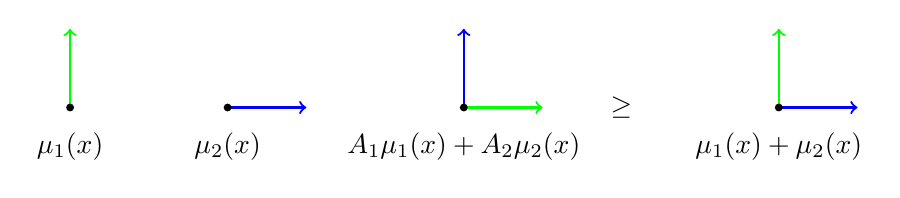
\begin{tikzpicture}
      \begin{scope}[shift={(-7,0)}]
        \draw[thick,->,green] (0,0) to (0,1);
        \fill (0,0) circle(.05);
        \node at (0,-.5) {$\mu_1(x)$};
      \end{scope}

      \begin{scope}[shift={(-5,0)}]
        \draw[thick,->,blue] (0,0) to (1,0);
        \fill (0,0) circle(.05);
        \node at (0,-.5) {$\mu_2(x)$};
      \end{scope}

      \begin{scope}[shift={(-2,0)}]
        \draw[thick,->,green] (0,0) to (1,0);
        \draw[thick,->,blue] (0,0) to (0,1);
        \fill (0,0) circle(.05);
        \node at (0,-.5) {$\pushf{A_{1}}{\mu_1(x)} + \pushf{A_{2}}{\mu_2(x)}$};
      \end{scope}

      \begin{scope}[shift={(0,0)}]
        \node at (0,0) {$\geq$};
      \end{scope}

      \begin{scope}[shift={(2,0)}]
        \draw[thick,->,green] (0,0) to (0,1);
        \draw[thick,->,blue] (0,0) to (1,0);
        \fill (0,0) circle(.05);
        \node at (0,-.5) {$\mu_1(x) + \mu_2(x)$};
      \end{scope}
    \end{tikzpicture}
    \caption{A representation of the optimal dual solution of \exemref{simple0} with the constraint \eqref{eq:dualinf1}.}
    \label{fig:simple0}
  \end{figure}

  A dual solution $\mu_1$ (resp. $\mu_2$)\footnote{In the arbitrary switching case, we write $\mu_\sigma$ instead of $\mu_{uv\sigma}$ for short}
  for the first (resp. second) matrix has the measure $\mu_1 = \delta_{(0,1)}/2$ (resp. $\mu_2 = \delta_{(1,0)}/2$).
  This is the solution obtained by applying \lemref{traj2meas} to the cycle $(1, 2)$.
  This is shown in \figref{simple0}.

\end{myexem}

\begin{myrem}
  Occupation measures for continuous switched systems are studied in \cite{claeys2016modal}.
  These measures are supported on the cartesian product of the state space and a finite interval of time $t \in [0, T]$
  while in this paper, the measures are only supported on the subset $\Sn$ of the state space.
  Indeed, since the system \eqref{eq:switchsys} is homogeneous and time-invariant, we can encode trajectories in a measure on $\Sn$ (\lemref{traj2meas}) and
  still be able to recover it (\cororef{instabcert}).

  The measures studied in \cite{hare2011explicit} are supported on the paths in $\G$.
  They are related to the measures studied in this paper since given a cycle $c$,
  we can compute the occupation measures of the trajectory using this switching cycle and starting with a leading eigenvector of $A_c$ as $x_0$ with \lemref{traj2meas}.
\end{myrem}



One may wonder whether \lemref{traj2meas} also works in the reverse direction to give a \emph{constructive} proof for \cororef{instabcert} when the measures $\mu_{uv\sigma}$ are atomic.
Namely, can we extract a periodic trajectory of period $c$ with $\jsrc \geq \gamlb$ from any atomic feasible solution of \progref{dualinf} with $\gamlb$.
As such solution may be the convex hull of solutions obtained by the construction of \lemref{traj2meas}, we may recover several periodic trajectory, from which there might be only one that satisfies $\jsrc \geq \gamlb$.
The following Lemma provides a constructive way to recover a periodic trajectory of period $c$ satisfying $\jsrc \geq \gamlb$ in the scalar case%
\footnote{Note that in this case, any measure is atomic since $\Sn$ is zero-dimensional}%
, i.e. $n = 1$%





\begin{lemma}
  \label{lem:instabcerts}
  Consider \defAGs{}.
  If there exists a feasible solution $\mu$ of \progref{dualinf} with $\gamlb$,
  then there exists a cycle $c$ with $\jsrc \geq \gamlb$.
  \begin{proof}
    Let $(\mu, \gamma)$ be the solution.
    By \eqref{eq:dualinf3} and \eqref{eq:dualinf1}, we can find a cycle $c$ for which each edge $e$ has a nonzero measure $\mu_e$.

    If $\jsrc \geq \gamma$, we are done.
    Otherwise, if $\jsrc < \gamma$, using \lemref{traj2meas},
    we can build a feasible solution $\nu$ such that \eqref{eq:dualinf1} is satisfied with equality for $\gamlb = \jsrc$.
    This means that $\mu - \lambda \nu$ is feasible with $\gamma$ for any $\lambda \geq 0$ such that $\mu - \lambda \nu \geq 0$.
    Let $\opt{\lambda}$ be the maximum value of $\lambda$ such that $\mu - \lambda \nu \geq 0$.
    Since $n = 1$, $\Sn$ is zero dimensional so for at least one edge $e$ of the cycle $c$, $\mu_e - \opt{\lambda} \nu_e$ is zero.
    Moreover, since $\mu_e$ is nonzero for all edge $e$ of the cycle, $\lambda > 0$.
    Therefore, the number of edges with nonzero measure has decreased and at least one of the constraints \eqref{eq:dualinf1} is now satisfied with strict inequality.

    This process can only be repeated finitely many times until $\mu$ becomes the trivial solution since the number of edges with nonzero measure decrease each time.
    Moreover we will have $\jsrc \geq \gamma$ at least once since the constraints \eqref{eq:dualinf1} cannot be satisfied with strict inequality for the trivial solution.
  \end{proof}
\end{lemma}

Given a feasible solution of \progref{dualinf} and a common partition of the support of the measures,
we show in \propref{Bsc} how to transform the solution into a solution of a scalar switched system.
Using this transformation, we can always recover a cycle $c$ for which $\jsrc = \gamma$ from a solution of \progref{dualinf} with $\gamlb = \gamma$ for which the measures are atomic.

\begin{proposition}
  \label{prop:Bsc}
  Consider \defAGe.
  Suppose that there exists a feasible solution $\mu$ of \progref{dualinf} with $\gamlb = \gamma$
  and a finite family $\mathcal{S}$ of disjoint subsets of $\Sn$ such that
  the support of each measure is included in the union of the sets of the family $\mathcal{S}$.
  Then there exists sets $B_1, \ldots, B_k \in \mathcal{S}$ and a cycle $\sigma_1, \ldots, \sigma_k$ of $\G$ such that
  \[ \prod_{i=1}^k \max_{x \in B_i} \|A_{\sigma_i} x\|_2 \geq \gamma^k \]
  and $A_{\sigma_i} B_i \cap B_{i+1} \neq \emptyset$ for $i=1, \ldots, k$ where $B_{k+1}=B_1$.
  \begin{proof}
    Given a set $B \in \mathcal{S}$ and an \arc{} $e \in \Arcs$, let $\mu_e^B$ denote the measure defined as $\mu_e^B(C) = \mu_e(C \cap B)$.
    We consider a new constrained switched system with matrices $\A' \subseteq \R^{1 \times 1}$ and automaton $\G'(\Nodes', \Arcs')$
    where $\Nodes' = \{\, (v,B) \mid v \in \Nodes, B \in \mathcal{S} \,\}$,
    $e'((u,v,\sigma), B, C) = ((u,B), (v,C), (\sigma,B))$,
    $\Arcs' = \{ e'(e, B, C) \mid e \in \Arcs, B, C \in \mathcal{S}, A_e B \cap C \neq \emptyset \}$,
    and $A'_{(\sigma,B)} = \max_{x \in B} \|A_\sigma x\|_2$.
    From any solution $\mu$ of the original system feasible for $\gamlb$, the following solution of the system with matrices $\A'$ and automaton $\G'$
    \[ \mu'_{e'(e,B,C)} = \frac{(\pushf{A_e}{\mu_e^B})(C)}{(\pushf{A_e}{\mu_e^B})(\Sn)} \mu_e(B) \]
    is also feasible with $\gamlb$.
    Indeed, by construction, for any $v \in \Nodes, C \in \mathcal{S}$, we have
    \begin{align}
        \label{eq:lhstransfer}
        \begin{split}
        \sum_{e \in \Arcsin_{1}(v), B \in \mathcal{S}} (\pushf{A_e}{\mu_e^B})(C)
        & =
        \sum_{e \in \Arcsin_{1}(v), B \in \mathcal{S}} \mu_{e'(e, B, C)}' \frac{(\pushf{A_e}{\mu_e^B})(\Sn)}{\mu_e(B)}\\
        & \stackrel{\eqref{eq:pushfineq}}{\leq}
        \sum_{e \in \Arcsin[\Arcs']_1(v, C)} \pushf{A'_{e}}{\mu_{e}'}
        \end{split}\\
        \label{eq:rhstransfer}
        \begin{split}
        \sum_{e \in \Arcsout_1(v)} \mu_e(C)
        & =
        \sum_{e \in \Arcsout_1(v), D \in \mathcal{S}} \frac{(\pushf{A_e}{\mu_e^C})(D)}{(\pushf{A_e}{\mu_e^C})(\Sn)} \mu_e(C)\\
        & =
        \sum_{e \in \Arcsout[\Arcs']_1(v, C)} \mu_{e}'.
        \end{split}
    \end{align}
    By \eqref{eq:dualinf1} on $\mu$, the left-hand side of \eqref{eq:rhstransfer} is smaller than
    the left-hand side of \eqref{eq:lhstransfer}.
    Therefore, the right-hand side of \eqref{eq:rhstransfer} is smaller than the right-hand side of \eqref{eq:lhstransfer}
    hence $\mu'$ satisfies \eqref{eq:dualinf1} on the new switched system.

    Therefore, by \lemref{instabcerts},
    there is a cycle $(\sigma_1, B_1), \ldots, (\sigma_k, B_k)$ of $\G'$ such that the modes $\sigma_i$ and sets $B_i$ are as required.
  \end{proof}
\end{proposition}

\begin{myexem}
  \label{exem:simple05}
  Consider the dual solution obtained in \exemref{simple0}.

  The supports of $\mu_1$ and $\mu_2$ are respectively $B_1 = \{(0, 1)\}$ and $B_2 = \{(1, 0)\}$.
  The automaton $G'(V', E')$ obtained by the transformation of \propref{Bsc} is defined by
  $V' = \{(1, B_1), (1, B_2)\}$ and $E' = \{((1, B_1), (1, B_2), (1, B_1)), ((1, B_2), (1, B_1), (2, B_2))\}$.
  The new $1 \times 1$ matrices are $A'_{(1, B_1)} = 1$ and $A'_{(2, B_2)} = 1$.

  The computation of the CJSR of this scalar system is a \emph{maximum cycle mean} problem
  as outlined in \cite{ahmadi2012joint}.
  The cycle of maximum geometric mean is $((1, B_1), (2, B_2))$ which geometric mean $\sqrt{1 \cdot 1} = 1$.
  We recover the cycle $(1, 2)$ found in \exemref{simple0}.
\end{myexem}


\section{Automaton-dependent bounds}
In this section, we introduce a method to approximate the CJSR using SOS programming and provide a new guarantee relating its accuracy with the spectral radius of the adjacency matrix and the $p$-radius; the definition of the $p$-radius can be found in the \appref{pradius}.
\label{sec:primal}


\subsection{Sum of squares programming}
\label{sec:sosprog}
Deciding whether a multivariate polynomial of degree $2d \geq 4$ is nonnegative is known to be NP-hard.
However a sufficient condition for a polynomial to be nonnegative is easy to check.
We say that a polynomial is a \emph{sum of squares} (SOS) if there exist
polynomials $q_1, \ldots, q_M$ such that
\[ p(x) = \sum_{k=1}^Mq_k^2(x). \]
If a polynomial is SOS, then it is obviously nonnegative.

It is well known that if $p(x)$ is an homogeneous polynomial of degree
$2d$ then each $q_k(x)$ must be an homogeneous polynomial of degree $d$;
this can be shown easily using the Newton polytope of $p(x)$ and
\cite[Theorem~1]{reznick1978extremal}.  Let $x^{[d]}$ represent a
basis of the homogeneous polynomials of degree $d$.  We can check
whether a polynomial is SOS using semidefinite programming thanks to
the following theorem.
\begin{theorem}[\cite{choi1995sums,nesterov2000squared,parrilo2000structured,parrilo2003semidefinite,shor1987class}]
  \label{theo:sos}
  A homogeneous multivariate polynomial $p(x)$ of degree $2d$ is a sum
  of squares if and only if
  \[ p(x) = (x^{[d]})^\Tr Q x^{[d]} \]
  where $Q$ is a symmetric positive semidefinite matrix.
\end{theorem}

From the exact arithmetic viewpoint, the basis $x^{[d]}$ chosen in \theoref{sos} does
not affect whether $p(x)$ is SOS or not.  A specific choice of basis
may however improve the numerical behaviour of the corresponding
semidefinite program.

We denote the set of homogeneous polynomials of degree $2d$ as
$\Rh[x]$, the cone of homogeneous SOS polynomials of degree $2d$ as
$\Sosh$ and the dual of $\Sosh$ as $\Soshd$.

A common interpretation of the dual space $\Rhd$ of linear functionals on homogeneous polynomials of degree $2d$ is the space of moments of momonials of degree $2d$.
If $p(x) = a^\Tr x^{[d]}$ and $m$ is the vector of moments of $x^{[d]}$ of a measure $\mu$ then
\[ \la m, a \ra = \int p(x) \dif \mu = \la \mu, p \ra. \]
As a sum of squares polynomial is nonnegative,
this integral is nonnegative for any measure $\mu$.
Therefore, given a moment vector $m$, a necessary condition for a measure to exist with these moments is that $\la m, a \ra \geq 0$ for any vector of coefficients $a$ of a sum of squares polynomial.
That is, $\Soshd$ is a superset of the set of moments of measures.
The members of $\Soshd$ are often called \emph{pseudo-measures} and denoted $\pmu$; see~\cite{barak2012hypercontractivity}.


\subsection{CJSR Approximation via SOS}
\label{sec:sos}

The $2d$th root of homogeneous polynomials of degree $2d$ can be used as Lyapunov function.
\begin{proposition}
  \label{prop:pos}
  Consider \defAGe{}.
  Suppose that there exist $|\Nodes|$ strictly positive homogeneous polynomials $p_v(x)$ of degree $2d$
  such that
  \[ p_{v}(A_\sigma x) \leq \gamub^{2d}p_{u}(x) \]
  holds for all \arc{} $(u,v,\sigma) \in \Arcs$.
  Then $\cjsr \leq \gamub$.
  \begin{proof}
    Define $f_v(x) = [p_v(x)]^{\frac{1}{2d}}$ and use \theoref{stabcert}.
  \end{proof}
\end{proposition}

We relax the positivity condition of \propref{pos} by the more tractable sum of squares (SOS) condition and
define $\jsrsos$ as the solution of the following SOS restriction of \progref{primalinf}.
\begin{myprog}[Primal]
  \label{prog:primal}
  \begin{align}
    \notag
    \inf_{p_v(x) \in \Rh[x],\gamub \in \R} \gamub\\
    \notag
    \gamub^{2d} p_u(x) - p_v(A_\sigma x) & \text{ is SOS}, \quad \forall (u, v, \sigma) \in \Arcs,\\
    \label{eq:soscons1}
    p_v(x) & \text{ is SOS}, \quad \forall v \in \Nodes,\\
    \label{eq:soscons3}
    p_v(x) & \text{ is strictly positive}, \quad \forall v \in \Nodes,\\
    \notag
    \sum_{v \in V} \int_{\mathbb{S}^{n-1}} p_v(x) \dif x & = 1.
  \end{align}
\end{myprog}

\begin{myrem}
  In practice we can replace \eqref{eq:soscons1} and \eqref{eq:soscons3} by ``$p_v(x) - \epsilon\|x\|_2^{2d}$ is SOS''
  for any $\epsilon > 0$.
  This constrains $p_v(x)$ to be in the interior of the SOS cone,
  which is sufficient for $p_v(x)$ to be strictly positive.
  The bounds given in \Sect\ref{sec:quality} are valid
  if $p_v(x)$ is in the interior of the SOS cone.
\end{myrem}

By \propref{pos},
a feasible solution of Program~\ref{prog:primal} gives an upper bound for $\cjsr$,
and thus, for any positive degree $2d$,
\begin{equation}
  \label{eq:upperbound}
  \cjsr \leq \jsrsos.
\end{equation}


\begin{myexem}
  \label{exem:simple1}
  Consider the unconstrained system \cite[Example~2.1]{ahmadi2012joint} with $m=3$:
  \[ \A = \{ A_1 = e_1e_2^\Tr , A_2 = e_2e_3^\Tr , A_3 = e_3e_1^\Tr  \} \]
  where $e_i$ denotes the $i$th canonical basis vector.

  One can verify that for any $d$, a solution to Program~\ref{prog:primal} is given by
  \[ (p(x), \gamma) = (x_1^{2d} + x_2^{2d} + x_3^{2d}, 1). \]
\end{myexem}

\begin{myexem}
  \label{exem:run2}
  Let us reconsider our running example; see Example~\ref{exem:run1}.
  The optimal solution of Program~\ref{prog:primal}
  is represented by
  Figure~\ref{fig:primal} for $2d = 2$, 4, 6, 8, 10 and 12.
  \begin{figure}[!ht]
    \centering
    \tabulinesep=0.5mm
    \begin{tabu}{{X[0.85,c,m]X[c,m]X[c,m]X[c,m]X[c,m]}}
      & Node 1 & Node 2 & Node 3 & Node 4\\
      \PrimalFig{2}{1}
      \PrimalFig{4}{2}
      \PrimalFig{6}{3}
      \PrimalFig{8}{4}
      \PrimalFig{10}{5}
      \PrimalFig{12}{6}
    \end{tabu}
    \caption{
    Representation of the solutions to Program~\ref{prog:primal}
    with different values of $d$ for the running example.
    The blue curve represents the boundary of the
    1-sublevel set of the optimal
    solution $p_v$ at each node $v \in \Nodes$.
    The dashed curve is the boundary of the unit circle.
    Observe that some sets are not convex.}
    \label{fig:primal}
  \end{figure}
\end{myexem}



\subsection{Approximation guarantees}
\label{sec:quality}
In this section, we provide a new bound that relates the accuracy of Program~\ref{prog:primal} to the $p$-radius and the spectral radius of the adjacency matrix of the automaton.
The $p$-radius is a generalization of the joint spectral radius;
we recover the JSR with $p=\infty$.
The definition of the $p$-radius and its property can be found in \appref{pradius}; see \cite{jungers2011fast} for an introduction.

An important property of the $p$-radius is that it is increasing in $p$.
\begin{lemma}
  \label{lem:incp}
  Consider \defAG{}.
  For any integers $p \leq q$,
  \begin{equation}
    \label{eq:incp}
    \cpr[p] \leq \cpr[q] \leq \cjsr \leq \rho(A(\G))^{\frac{1}{q}}
    \cpr[q] \leq \rho(A(\G))^{\frac{1}{p}} \cpr[p].
  \end{equation}
\end{lemma}
The proof can be found in \appref{pradius}.
This Lemma is already known in the unconstrained case~\cite{zhou2002p}.

\begin{myrem}
  \lemref{incp} shows that the $p$-radius provides an upper and lower bound on the CJSR.
  It is known that the $2d$-radius can be computed
  either by computing a spectral radius~\cite{blondel2005computationally}
  or by solving a linear program~\cite{parrilo2008approximation}
  (see \cite{ogura2016efficient} for computation algorithms when $p$ is not an even integer).
  One needs to do either of these two operations on
  either the sum of the $d$th Kronecker power of the veronese 2-lift of the matrices
  or the sum of the veronese $2d$-lift of the matrices.
  However, the size of the matrices obtained by taking the $d$th Kronecker power grows rapidly
  and the veronese lifting needs to compute permanents which is computationally very demanding.
  Usually, for the same $d$, \progref{primal} gives approximations of the CJSR with a much higher accuracy at the cost of solving an SDP on smaller matrices.
  While solving an SDP is more demanding than computing a spectral radius or solving a linear program, since the matrices are smaller than with the Kronecker powering
  and we do not need to compute permanents, this method is actually more scalable.
\end{myrem}


In this section, we show the following bound stating that the solution found by \progref{primal} is at least as good as the bound obtained by computing the $2d$-radius.
\begin{theorem}
  \label{theo:second}
  Consider \defAG{} and a positive integer $d$.
  The approximation given by \progref{primal} using homogeneous polynomials of degree $2d$
  satisfies:
  \begin{equation}
    \label{eq:second}
    \jsrsos \leq \rho(A(\G))^{\frac{1}{2d}}\cdr \leq \rho(A(\G))^{\frac{1}{2d}} \cjsr
  \end{equation}
  where $A(\G)$ is the adjacency matrix of $\G$.
\end{theorem}
Note that the second inequality in \eqref{eq:second} is simply \eqref{eq:incp}.
This theorem is proved at the end of this section.

As a corollary of Theorem~\ref{theo:second}, in the trivial cases such that $\rho(A(\G)) = 1$, the approximation is exact.
This corresponds to the case where every node of $\G$ has indegree and outdegree 1.
In that case, the graph forms a cycle of some length $k$ and the CJSR is simply the $k$th root of the spectral radius of the product of the matrices along this cycle.

In the general case, the following approximation guarantee is known (note that the bound does not take into account the particular structure of the automaton):
\begin{theorem}[{\cite[Theorem~3.6]{philippe2016stability}}]
  \label{theo:matt}
  Consider \defAGn{} and a positive integer $d$.
  The approximation $\jsrsos$ given by Program~\ref{prog:primal} using homogeneous polynomials of degree $2d$
  satisfies:
  \[ \jsrsos \leq {n+d-1 \choose d}^{\frac{1}{2d}} \cjsr. \]
\end{theorem}

The results of \theoref{second}, \theoref{matt} and \eqref{eq:upperbound} are summarized by the following corollary.
\begin{corollary}
  \label{coro:mix}
  Consider \defAGn{} and a positive integer $d$,
  the approximation given by Program~\ref{prog:primal} using homogeneous polynomials of degree $2d$
  satisfies:
  \[
    \min\Big\{{n+d-1 \choose d}, \rho(A(\G))\Big\}^{-\frac{1}{2d}} \jsrsos%
    \leq \cjsr \leq \jsrsos
  \]
  where $A(G)$ is the adjacency matrix of the automaton $\G$.
\end{corollary}
We see that we can have arbitrary accuracy by increasing $d$.

For the arbitrary switching case, $\rho(A(\G))$ is equal to the number of matrices $m$.
Theorem~\ref{theo:second} was already known in this particular case \cite[Theorem~4.3]{parrilo2008approximation}.

Our proof technique relies on the analysis of an iteration in the vector space of polynomials of degree $2d$.
When this iteration converges, it converges to a feasible solution of Program~\ref{prog:primal}.
By analysing this iteration as affine iterations in this vector space, we derive a sufficient condition for its convergence
and thus an upper bound for $\jsrsos$.

Consider the iteration
\begin{align}
  \notag
  p_{v,0}(x) & = 0,\\
  \label{eq:iter}
  p_{v,k+1}(x) & = q_v(x) + \frac{1}{\iterc} %
  \sum_{(u,v,\sigma) \in \Arcs} p_{u,k}(A_\sigma x), \quad  v \in \Nodes
\end{align}
for fixed homogeneous polynomials $q_v(x)$ of degree $2d$ in $n$ variables (not necessarily different)
and a constant $\iterc > 0$.

When this iteration converges, it converges to a feasible solution of Program~\ref{prog:primal}.
\begin{lemma}
  \label{lem:conv}
  Consider a constant $\iterc > 0$.
  If there exist homogeneous polynomials $q_v(x)$ in the interior of the SOS cone such that
  iteration~\eqref{eq:iter} converges then
  \[
    \jsrsos \leq \iterc^{\frac{1}{2d}}.
  \]
  \begin{proof}
    Suppose the iteration converges to the polynomials $p_{v,\infty}(x)$.
    It is easy to show by induction that $p_{v,k}(x)$ is SOS for all $k$.
    It is trivial for $k = 0$ and if it is true for $k$ then it is also true for $k+1$ by \eqref{eq:iter}.
    Since the SOS cone is closed, $p_{v,\infty}$ is SOS.
    Now by \eqref{eq:iter}, for each $v \in \Nodes$,
    \[ p_{v,\infty}(x) = q_v(x) + \frac{1}{\iterc} %
    \sum_{(u,v,\sigma) \in \Arcs} p_{u,\infty}(A_\sigma x) \]
    so $p_{v,\infty}(x)$ is also in the interior of the SOS cone.
    For each edge $(u,v,\sigma)$, by manipulating the above equation, we have
    \[ \iterc p_{v,\infty}(x) - p_{u,\infty}(A_\sigma x) = \iterc q_v(x) + %
    \sum_{(u',v',\sigma') \in \Arcs} p_{u',\infty}(A_{\sigma'} x) \]
    so $\iterc p_{v,\infty}(x) - p_{u,\infty}(A_\sigma x)$ is SOS.
    Therefore $(\{\, p_{v,\infty}(x) : v \in \Nodes \,\}, \iterc^{\frac{1}{2d}})$ is a feasible solution of Program~\ref{prog:primal}.
  \end{proof}
\end{lemma}

In view of \lemref{conv}, it is thus natural to analyse
under which condition iteration~\ref{eq:iter} converges. Recall
that iteration~\ref{eq:iter} is an affine map on the vector space of
homogeneous polynomials of degree $2d$.

\begin{proof}[Proof of Theorem~\ref{theo:second}]
  Iteration~\ref{eq:iter} is an affine map on the vector space of
  homogeneous polynomials of degree $2d$.  It is well known that
  if the convergence is guaranteed when we only retain the linear
  part of the affine map then it is also guaranteed for the affine
  iteration.

  Therefore we can analyse instead the following iteration
  \begin{align*}
    p_{v,0}(x) & = q_v(x),\\
    p_{v,k+1}(x) & = \frac{1}{\iterc} %
    \sum_{(u,v,\sigma) \in \Arcs} p_{u,k}(A_\sigma x), \quad  v \in \Nodes
  \end{align*}

  We can see that
  \begin{equation}
    p_{v,k+1}(x) = \frac{1}{\iterc^k}\sum_{s \in \Arcsin_k(v)} q_{s(1)}(A_s x)\\
    \leq \frac{1}{\iterc^k}\sum_{s \in \Arcsin_k(v)} q_{s(1)}(A_s x).
  \end{equation}

  Consider a norm $\|\cdot\|$ of $\R^n$ and its corresponding induced matrix norm of $\R^{n \times n}$.
  For each $v \in \Nodes$, we know by continuity of $q_v(x)$ that there exist $\beta_v > 0$ such that
  \[ q_v(x) \leq \beta_v\|x\|^{2d} \]
  for all $x \in \R^n$.
  Let $\beta = \max_{v \in \Nodes} \beta_v$.

  Therefore,
  \begin{align*}
    p_{v,k+1}(x)
    & \leq \frac{1}{\iterc^k}\sum_{s \in \Arcsin_k(v)} \beta_v \|A_s\|^{2d} \|x\|^{2d}\\
    & \leq \frac{\beta}{\iterc^k} \|x\|^{2d} \sum_{s \in \Arcsin_k(v)} \|A_s\|^{2d}.
  \end{align*}
  By Lemma~\ref{lem:rhoAG} and Remark~\ref{rem:path}, if
  $\iterc > \rho(A(G))\cdr^{2d}$, $\lim_{k \to \infty} p_{v,k}(x) = 0$.
  We obtain the result by \lemref{conv}.
\end{proof}


\section{Finding high-growth sequences}
\label{sec:dualalgo}
In \secref{sos}, we introduced the SOS restriction of \progref{primalinf} with \progref{primal}.
In this section, we introduce \progref{dual}, the moment relaxation of \progref{dualinf}.
It turns out that \progref{primal} and \progref{dual} are dual to each other.
Indeed, the proof of \lemref{duality} can be translated verbatim in order to prove that \progref{dual} is the dual of \progref{primal}.


\subsection{Dual SOS program}
\label{sec:dual}




\begin{myprog}[Dual of \progref{primal}]
  \label{prog:dual}
  \begin{align}
    \notag
    \sup_{\pmu_{uv\sigma} \in \Rhd, \gamlb \in \R} \gamlb\\
    \label{eq:dual1}
    \sum_{(u,v,\sigma) \in \Arcs} \pushf{A_\sigma}{\pmu_{uv\sigma}} - \gamlb^{2d} \sum_{(v,w,\sigma) \in \Arcs} \pmu_{vw\sigma} & \in \Soshd, \forall v \in \Nodes,\\
    \label{eq:dual2}
    \pmu_{uv\sigma} & \in \Soshd, \quad \forall (u,v,\sigma) \in \Arcs,\\
    \label{eq:dual3}
    \sum_{(u,v,\sigma) \in \Arcs} \pmu_{uv\sigma}(\Sn) & = 1.
  \end{align}
\end{myprog}





It is important to note that a solution of \progref{dual} is not necessarily a solution of \progref{dualinf}.
First $\pmu_{uv\sigma}$ may not be a measure even if it belongs to $\Soshd$ as discussed in \secref{sosprog}.
Second, the left-hand side of \eqref{eq:dual1} may also not be a measure.
For this second concern, it helps to be more explicit.
Suppose for instance that we are in the quadratic case, i.e. $d = 1$.
In that case, if $\pmu \in \Soshd[2]$, there always exists a measure $\mu$ that has the moments of the pseudo-measure $\pmu$.
We can take for instance a Gaussian distribution with these second order moments.
Hence we can find Gaussian distributions $\mu_{uv\sigma}$ that have the second order moments $\pmu_{uv\sigma}$
and Gaussian distributions $\nu_v$ that have the second order moments given by the left-hand side of \eqref{eq:dual1}.
However, we may have
\[ \sum_{(u,v,\sigma) \in \Arcs} \pushf{A_\sigma}{\mu_{uv\sigma}} - \gamlb^{2d} \sum_{(v,w,\sigma) \in \Arcs} \mu_{vw\sigma} \neq \nu_v \]
as we only know that the left-hand side and right-hand side of the above equation have the same second order moments;
see \exemref{run3}.

However, in some cases, we can recover a feasible solution of \progref{dualinf} from a feasible solution of \progref{dual}.
In these cases, by \cororef{instabcert}, this provides a lower bound on the CJSR.
Moreover, there exist efficient techniques allowing to detect situations where the solution is moments of an atomic measure; see \cite{henrion2005detecting, laurent2009sums}.
Then, using the transformation of \propref{Bsc}, we can transform
these atomic measures into a feasible solution of a constrained scalar switched systems.
For such system, we could use the algorithm described in \lemref{instabcerts} but as pointed out in \cite{ahmadi2012joint},
computing the CJSR of a scalar system can easily be done by solving a maximum cycle mean problem for which efficient algorithm exists \cite{karp1978characterization}.

If we recover a feasible solution of \progref{dualinf} from a feasible solution of \progref{dual} with $\gamlb = \jsrsos$,
we can directly conclude that $\jsrsos = \cjsr$.
This is somewhat similar to the minimization of a multivariate polynomial using SOS where we can detect that we have reached the optimum
when the measure is atomic and recover the minimizers of the polynomial from the atoms of the measure. %

However, we may also check for atomic feasible solutions of \progref{dualinf} with $\gamlb < \jsrsos$ to provide lower bounds.
Moreover, in practice, $\jsrsos$ is computed by binary search on $\gamlb$ so we often have several such solutions.

\begin{myexem}
  \label{exem:simple2}
  Consider \exemref{simple1}.
  For $i = 1, 2, 3$, let $\pmu_i$ be the solution of \progref{dual} corresponding to the matrix $A_i$.
  For any $d$, we can see that the dual solution for $\gamma = 1$ is such that
  the only monomial $x^\alpha$ such that $\la\pmu_1, x^\alpha \ra$ (resp. $\la \pmu_2, x^\alpha \ra$, $\la \pmu_3, x^\alpha \ra$) is non-zero is $x_1^{2d}$ (resp. $x_2^{2d}$, $x_3^{2d}$)
  and $\la \pmu_1, x_1^{2d} \ra = \la \pmu_2, x_2^{2d} \ra = \la \pmu_3, x_3^{2d} \ra = 1/3$.
  Note that it means that $\pmu_1 = \delta_{(1,0,0)}/3$, $\pmu_2 = \delta_{(0,1,0)}/3$ and $\pmu_3 = \delta_{(0,0,1)}/3$
  where $\delta_x$ is the Dirac measure centered on $x$.
  Since these measures are solution to \progref{dualinf} with $\gamlb = 1$,
  by \cororef{instabcert}, this means that $\jsr \geq 1$.
\end{myexem}


\begin{myexem}
  \label{exem:run3}
  We continue the running example; see Example~\ref{exem:run1} and Example~\ref{exem:run2}.

  For all $d$, $\pmu_{212} = \pmu_{323} = \pmu_{344} = \pmu_{431} = 0$
  hence the node 4 is ``unused'' by the dual.
  For $2d = 2, 4$, $\pmu_{123} = \pmu_{231} = 0$ so
  the node $2$ is ``unused'' for low degree.

  At first, one could think that the dual variables can be used to reduce the systems,
  e.g. remove nodes or edges.
  However, it would be a mistake to remove the node 2 since the periodic trajectory with highest growth rate uses this node.



  It is also interesting to notice that the matrices corresponding to the dual variables have low rank.
  For example, for $2d = 2$, $\pmu_{131}$
  (resp. $\pmu_{312}$, $\pmu_{331}$) is the Dirac measure $5.873 \cdot \delta_{(0.917,0.399)}$
  (resp. $3.966 \cdot \delta_{(0.875,0.485)}$, $6.704 \cdot \delta_{(0.757,-0.653)}$).
  However, this is not a feasible solution of \progref{dualinf}.
  Indeed,
  while \eqref{eq:dualinf1} is satisfied for \node{} 1 since
  $\pushf{A_2}{\delta_{(0.875,0.485)}}$ gives $\delta_{(0.917,0.399)}$,
  \eqref{eq:dualinf1} is not satisfied for \node{} 3 as
  $\pushf{A_1}{\delta_{(0.917,0.399)}}$ gives $\delta_{(0.999, -0.0271)}$ and
  $\pushf{A_1}{\delta_{(0.757,-0.653)}}$ gives $\delta_{(0.422, -0.906)}$.
\end{myexem}


\subsection{Generating high growth sequence}
\label{sec:algo}
In this section we give an algorithm that generates an infinite
sequence of matrices such that the asymptotic growth rate of the
product of the matrices is arbitrarily close to the CJSR.
Note that by \defref{cjsr}, this asymptotic growth rate must be
smaller than the CJSR.


Given an \arc{} $e \in \Arcs$, let $\pE_e[p(x)] = \la \pmu_e, p(x) \ra$.
Given a polynomial $p_0(x) \in \inte(\Sosh)$ and an initial edge $(v_1,v_0,\sigma_1)$,
the algorithm builds a $\G^\Tr$-admissible
sequence $(v_1,v_0,\sigma_1),\allowbreak(v_2,v_1,\sigma_2), \ldots$ such that
\begin{equation}
	\label{eq:thetak}
  \theta_k \eqdef \pE_{v_{k}v_{k-1}\sigma_k}[p_0(A_{\sigma_1} \cdots A_{\sigma_k}x)]
\end{equation}
remains ``large'' for increasing $k$.
As we will see, using \lemref{thetatoA},
this implies that $A_{\sigma_1} \cdots A_{\sigma_k}$ has a ``large'' norm.

\begin{lemma}[{\cite[Lemma~6]{legat2016generating}}]
  \label{lem:sosbound}
  For any polynomial $p(x) \in \inte(\Sosh)$,
  there exists a constant $\beta$
  such that for any matrix $A$,
  \[ \beta\|A\|_2^{2d} p(x) - p(Ax) \quad \text{is SOS} \]
  where $\|A\|_2 = \rho(A^\Tr A)^{1/2}$ is the Euclidean norm.
\end{lemma}

\begin{lemma}
  \label{lem:thetatoA}
  Let us consider a solution $(\, \pmu_e : e \in \Arcs \,)$ of \progref{dual}.
  For any polynomial $p(x) \in \inte(\Sosh)$,
  there exists a positive constant $\tau$
  such that for any matrix $A \in \R^{n \times n}$ and \arc{} $e \in \Arcs$,
  \[ \pE_e[p(A x)] \leq \tau \|A\|_2^{2d} \]
  \begin{proof}
    If all pseudo-expectations are zero, the result is trivially true.
    Therefore we can suppose that at least one is nonzero.
    By \lemref{sosbound}, there exists a constant $\beta > 0$ such that
    \[ \beta \|A\|_2^{2d}p(x) - p(Ax) \text{ is SOS}. \]
    Hence
    \[
      \pE_e[p(Ax)] \leq \beta \|A\|_2^{2d} \pE_e[p(x)].
    \]
    We obtain the result with the constant
    \(
    \tau = \beta \max_{e \in \Arcs} \pE_{e}[p(x)].
    \)
    Since at least one pseudo-expectation is nonzero and $p(x)$ is in
    the interior of the SOS cone, $\tau > 0$.
  \end{proof}
\end{lemma}



\begin{algorithm}[!ht]
  \caption{Generates a sequence of large asymptotic growth using paths of length $l$.}
  \label{algo:prodl}
  \begin{algorithmic}
    \STATE{Given a feasible solution $(\, \pmu_e : e \in \Arcs \,)$ of \progref{dual}}
    \STATE{Pick an arbitrary polynomial $p_0(x) \in \inte(\Sosh)$}
    \STATE{Pick an \arc{} $(v_0,v_{-1},\sigma_0) \in \Arcs$ such that $\pE_{v_0v_{-1}\sigma_0}[p_0(x)] > 0$}
    \FOR{$k = 0,l,2l,\ldots$}
    \STATE Pick $s \in \argmax_{s \in \Arcsin_l(v_{k})} \pE_{s[1]}[p_k(A_s x)]$
    \STATE Set $(v_{k+l},\sigma_{k+l},\ldots,\sigma_{k+1},v_k) \leftarrow s$
    \STATE Set $p_{k+1} \leftarrow p_k(A_s x)$
    \ENDFOR
  \end{algorithmic}
\end{algorithm}





\lemref{maxdegpathl} provides a guarantee on the growth rate of $\theta_k$, defined in \eqref{eq:thetak},
using the dual constraint~\eqref{eq:dual1}.

\begin{lemma}
  \label{lem:dualconsl}
  Given \defAG{}, %
  if $\pmu$ is a feasible solution of \progref{dual} then,
  for any edge $(\bar{u},\bar{v},\bar{\sigma}) \in \Arcs$,
  the following holds:
  \begin{equation}
    \label{eq:dualconsl}
    \sum_{s \in \Arcsin_k(\bar{u})} \pushf{A_s}{\pmu_{s[1]}} \succeq \gamma^{2dk} \pmu_{\bar{u}\bar{v}\bar{\sigma}}
  \end{equation}
  where $\pmu_1 \succeq \pmu_2$ denotes $\pmu_1 - \pmu_2 \in \Soshd$.
  \begin{proof}
    We prove \eqref{eq:dualconsl} by induction, the case of $k=0$ being trivial.
    Suppose that
    \begin{equation}
      \label{eq:indhyp}
      \sum_{s' \in \Arcsin_{k-1}(\bar{u})}\pushf{A_{s'}}{\pmu_{s'[1]}} \succeq \gamma^{2d(k-1)} \pmu_{\bar{u}\bar{v}\bar{\sigma}}.
    \end{equation}
    We can rewrite the left-hand side of \eqref{eq:dualconsl} as
    \begin{equation}
      \label{eq:splitdualconsl}
      \sum_{s \in \Arcsin_k(\bar{u})} \pushf{A_s}{\pmu_{s[1]}} = \sum_{s' \in \Arcsin_{k-1}(\bar{u})} \pushf{A_{s'}}{\sum_{(u,s'(1),\sigma) \in \Arcs} \pushf{A_\sigma}{\pmu_{us'(1)\sigma}}}.
    \end{equation}
    By \eqref{eq:dual1},
    \[
      \sum_{(u,s'(1),\sigma) \in \Arcs} \pushf{A_{\sigma}}{\pmu_{us'(1)\sigma}}
      \succeq \gamma^{2d} \sum_{(s'(1),w,\sigma') \in \Arcs} \pmu_{s'(1)w\sigma'}.
    \]
    Since the dual variables $\pmu_{s'(1)w\sigma'}$ of the right-hand side are in the dual of the SOS cone,
    and one of them is $\pmu_{s'[1]}$, we have
    \[
      \sum_{(u,s'(1),\sigma) \in \Arcs} \pushf{A_{\sigma}}{\pmu_{us'(1)\sigma}}
      \succeq \gamma^{2d} \pmu_{s'[1]}.
    \]
    Applying $\pushf{A_{s'}}{}$ on both sides and using \eqref{eq:splitdualconsl} gives
    \[
      \sum_{s \in \Arcsin_k(\bar{u})} \pushf{A_s}{\pmu_{s[1]}} \succeq \gamma^{2d} \sum_{s' \in \Arcsin_{k-1}(\bar{u})}\pushf{A_{s'}}{\pmu_{s'[1]}} \stackrel{\eqref{eq:indhyp}}{\succeq} \gamma^{2dk} \pmu_{\bar{u}\bar{v}\bar{\sigma}}.
    \]
  \end{proof}
\end{lemma}

\begin{lemma}
  \label{lem:maxdegpathl}
  Consider \defAGe{}.
  For any positive integers $d$ and $l$,
    using \progref{dual} with any $\gamma < \jsrsosa\\(\G,\A)$,
  \algoref{prodl} with paths of length $l$
  produces a $\G^\Tr$-admissible sequence
  $(v_1,v_0,\\\sigma_0),(v_2,v_1,\sigma_1), \ldots$ %
  for which the sequence of $\theta_k$ defined in \eqref{eq:thetak}
  satisfies the following inequality for all $k > 0$ multiple of $l$:
  \begin{equation*}
    \theta_{k}
    \geq \frac{\gamma^{2dl}}{\dink[l](v_{k-l+1})}
    \theta_{k-l}
  \end{equation*}
  \begin{proof}
    By \lemref{dualconsl},
    \begin{align*}
      \sum_{s \in \Arcsin_l(v_{k-l+1})} \pE_{s[1]}[p_{k-l}(A_s x)]
      & \geq \gamma^{2dl} \theta_{k-l}.
    \end{align*}
    Since the value of $s$ chosen by \algoref{prodl} maximises $\pE_{s[1]}[p_{k-l}(A_s x)]$,
    the left-hand side of the above inequality is smaller or equal to $\dink[l](v_{k-l+1})\theta_k$.
  \end{proof}
\end{lemma}


\theoref{fourth} translates the guarantee on $\theta_k$ to a guarantee on $A_{\sigma_1} \cdots A_{\sigma_k}$ using \lemref{thetatoA}.

\begin{theorem}
  \label{theo:fourth}
  Consider \defAGe{}.
  For any positive integer $d$ and $l$,
  using \progref{dual} with any $\gamma < \jsrsos$,
  \algoref{prodl} with paths of length $l$
  produces a $\G^\Tr$-admissible sequence
  $(v_1,v_0,\sigma_0), (v_2,v_1,\sigma_1), \ldots$ %
  that satisfies the following inequality for all $k \geq 1$:
  \begin{equation*}
    \lim_{k \to \infty} \|A_{s_k}\|_2^\frac{1}{k} \geq \frac{\gamma}{\|(A(\G)^\Tr)^l\|_\infty^\frac{1}{2dl}}
  \end{equation*}
  where $s_k = (\sigma_k, \ldots, \sigma_1)$.
  \begin{proof}
    By \lemref{maxdegpathl}, for any $k$ multiple of $l$, %
    \begin{equation*}
      \pE_{s_k[1]}[p_0(A_{s_k}x)] \geq \frac{\gamma^{2dk}}{(\mdin_l)^\frac{k}{l}} \pE_{v_0v_{-1}\sigma_0}[p_0(x)]
    \end{equation*}

    By Lemma~\ref{lem:thetatoA},
    there exists a constant $\tau > 0$ such that
    \[
      \pE_{s_k[1]}[p_0(A_{s_k} x)] \leq \tau \|A_{s_k}\|^{2d}.
    \]

    Combining these two inequalities, we obtain
    \begin{align*}
      \tau \|A_{s_k}\|^{2d} & \geq \frac{\gamma^{2dk}}{(\mdin_l)^\frac{k}{l}} \pE_{v_0v_{-1}\sigma_0}[p_0(x)].
    \end{align*}
    Since $\pE_{v_0v_{-1}\sigma_0}$ is nonzero, $\pE_{v_0v_{-1}\sigma_0}[p_0(x)] > 0$.
    Therefore taking the $(2dk)$th root and the limit $k \to \infty$
    we obtain the result.
  \end{proof}
\end{theorem}


Taking the limit $l \to \infty$ and using \eqref{eq:rhoAG}, we see
that Theorem~\ref{theo:second} is a corollary of
Theorem~\ref{theo:fourth}.



\begin{myexem}
  \label{exem:simple3}
  Suppose that we apply Algorithm~\ref{algo:prodl} with $l = 1$ to \exemref{simple2}
  and let us denote by $c_\alpha$ the coefficient of the monomial $x^\alpha$ in the polynomial $p_0(x)$ chosen arbitrarily by the algorithm.
  The start of the sequence produced depends on the order between
  the coefficients $c_{(2d,0,0)},\allowbreak c_{(0,2d,0)},\allowbreak c_{(0,0,2d)}$.
  If $c_{(2d,0,0)}$ is the largest then
  the $\G$-admissible left-infinite sequence found is
  \( \ldots,1,2,3,1,2,3,1,2,3. \)

  The product $A_{\sigma_1} A_{\sigma_2} A_{\sigma_3} \cdots = A_3A_2A_1A_3A_2A_1 \cdots $
  is periodic and has an asymptotic growth rate $\rho(A_{\sigma_1}A_{\sigma_2}A_{\sigma_3})^{1/3}\allowbreak = 1$.
  Hence $1 \leq \cjsr$.
\end{myexem}


\begin{figure}[!ht]
  \begin{subfigure}{0.48\textwidth}
  \centering
    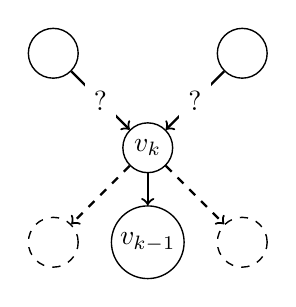
\begin{tikzpicture}
      \SetGraphUnit{1.2}
      \GraphInit[vstyle=Dijkstra]
      \SetVertexNoLabel
      \SetUpEdge[style={->}]
      \Vertex[NoLabel=false,L=$v_k$]{0}
      \NOWE(0){4};
      \NOEA(0){5};
      \SO[NoLabel=false,L=$v_{k-1}$](0){11};
      \tikzset{VertexStyle/.append style = {dashed}}
      \SOWE(0){10};
      \SOEA(0){12};
      \Edge[label=?](4)(0);
      \Edge[label=?](5)(0);
      \Edge(0)(11);
      \tikzset{EdgeStyle/.append style = {dashed}}
      \Edge(0)(10);
      \Edge(0)(12);
    \end{tikzpicture}
    \caption{One iteration of Algorithm~\ref{algo:prodl} with $l = 1$.}
    \label{fig:path1}
  \end{subfigure}
  \begin{subfigure}{0.48\textwidth}
  \centering
    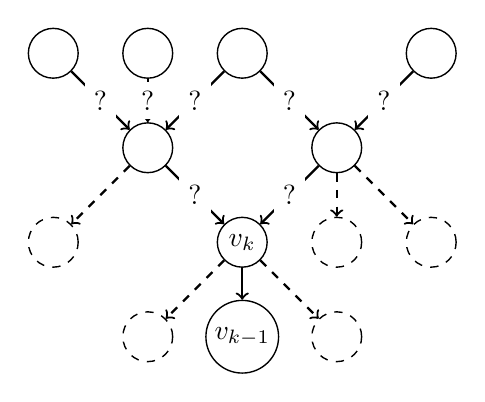
\begin{tikzpicture}
      \SetGraphUnit{1.2}
      \GraphInit[vstyle=Dijkstra]
      \SetVertexNoLabel
      \SetUpEdge[style={->}]
      \Vertex[NoLabel=false,L=$v_k$]{0}
      \NOWE(0){4};
      \NOEA(0){5};
      \NOWE(4){6};
      \NO  (4){7};
      \NOEA(4){8};
      \NOEA(5){9};
      \SO[NoLabel=false,L=$v_{k-1}$](0){11};
      \tikzset{VertexStyle/.append style = {dashed}}
      \SOWE(4){1};
      \EA(0){2};
      \EA(2){3};
      \SOWE(0){10};
      \SOEA(0){12};
      \Edge[label=?](6)(4);
      \Edge[label=?](7)(4);
      \Edge[label=?](8)(4);
      \Edge[label=?](8)(5);
      \Edge[label=?](9)(5);
      \Edge[label=?](4)(0);
      \Edge[label=?](5)(0);
      \Edge(0)(11);
      \tikzset{EdgeStyle/.append style = {dashed}}
      \Edge(4)(1);
      \Edge(5)(2);
      \Edge(5)(3);
      \Edge(0)(10);
      \Edge(0)(12);
    \end{tikzpicture}
    \caption{One iteration of Algorithm~\ref{algo:prodl} with $l = 2$.}
    \label{fig:path2}
  \end{subfigure}
  \caption{Comparison between Algorithm~\ref{algo:prodl} with $l = 1$ and $l = 2$.
  The solid edge denotes the the edge $(v_k, v_{k-1}, \sigma_k)$
  and the edges with question marks denote the incoming path considered by the iteration of the algorithm.}
  \label{fig:paths}
\end{figure}



\subsection{Producing lower bounds}
\label{sec:lb}


By definition of the CJSR, the asymptotic growth rate of the norm of the product of any $\G$-admissible (or $\G^\Tr $-admissible) sequence of matrices gives a lower bound on the CJSR.
In particular the sequence produced by Algorithm~\ref{algo:prodl} provides a lower bound on the CJSR.

If there are two integers $\bar{k},k$ such that the sequence after $\bar{k}$ is periodic of period $k$,
the asymptotic growth rate of the norm is equal to the $k$th root of the spectral radius of the product of the matrices of one period.
This is due to the Gelfand's formula $\rho(A) = \lim_{k \to \infty} \|A^k\|^{1/k}$.
From the same identity,
we see that the spectral radius of the product of the matrices of one $\G$-admissible cycle gives a lower bound on the CJSR.



To find lower bounds for the CJSR,
one could generate all the cycles of length smaller than some maximum length
and compute the spectral radius for all of them.
This brute force approach is not scalable because the number of paths considered grows exponentially with the maximum length.%
\footnote{The exponential growth of the brute force approach is the reason why one should choose a small $l$ for Algorithm~\ref{algo:prodl}.}

Gripenberg~\cite{gripenberg1996computing} proposes a branch-and-bound algorithm that prunes the search using an a priori fixed absolute error.
Two other branch-and-bound variant exists:
the balanced complex polytope algorithm \cite{guglielmi2008algorithm}
and the invariant conitope algorithm~\cite{jungers2014lifted}.

These algorithms can also be used to produce a $\G$-admissible sequence of matrices of high asymptotic growth rate
by reproducing the cycles of high spectral radius infinitely.
The advantage of Algorithm~\ref{algo:prodl} is that it provides a guarantee of accuracy given in \theoref{fourth}.
Algorithm~\ref{algo:prodl} provides at the same time a high growth infinite trajectory and lower bounds of guaranteed accuracy.

We can compute lower bounds using the upper bound provided by Program~\ref{prog:primal} and Corollary~\ref{coro:mix}
but in practice the trajectories are periodic after some time $\bar{k}$ so we are able to compute
much better lower bounds than the pessimistic bound provided by Corollary~\ref{coro:mix}.
This is shown by the following example.

\begin{myexem}
  \label{exem:run4}
  We tried the atom extraction procedure and Algorithm~\ref{algo:prodl} for $l = 1$ and $l = 3$ on our running example;
  see Example~\ref{exem:run1}, Example~\ref{exem:run2} and Example~\ref{exem:run3}.
  The code used to obtain the results of this example can be found on the author's website. %
  The result is shown in \figref{pedj}.
  We showed in \cite{legat2016generating} that the CJSR of the system is equal to 0.97482.
  We can see that this lower bound is found for $d = 4$ for $l=1$ and for $d=1$ for $l=3$.
  The atom extraction finds the lower bound 0.939255.
\end{myexem}

\begin{figure}[!ht]
  \begin{subfigure}{0.48\textwidth}
    \centering
    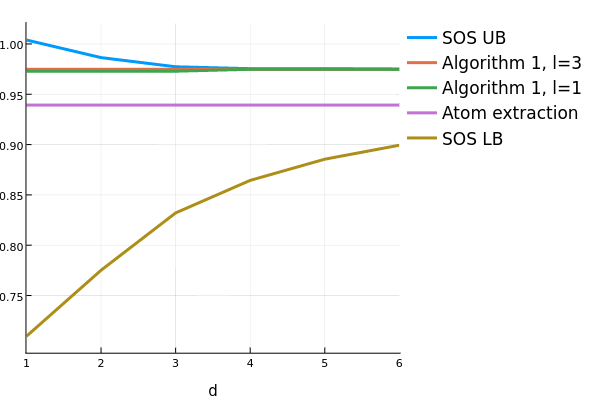
\includegraphics[width=\textwidth]{../../latex/images/PEDJ.png}
  \end{subfigure}
  \begin{subfigure}{0.48\textwidth}
    \centering
    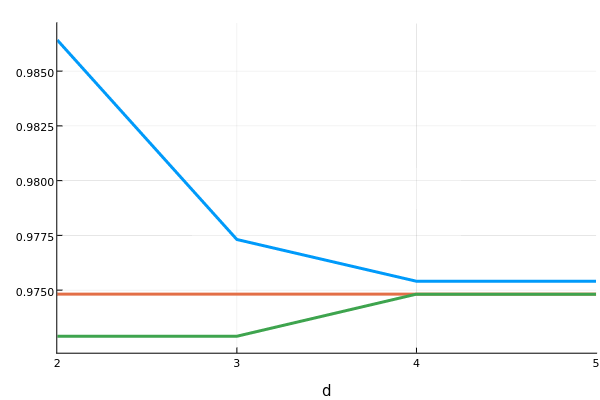
\includegraphics[width=\textwidth]{../../latex/images/PEDJ_zoom.png}
  \end{subfigure}
  \caption{Result of \exemref{run4}. The SOS UB is the upper bound found by \progref{primal} and the SOS LB is obtained from this upper bound the guarantee given in \cororef{mix}. The value $d$ of horizontal axis corresponds to using polynomials of degree $2d$. The right figure is a zoom of the left figure.}
  \label{fig:pedj}
\end{figure}



\subsection{Improving the automaton-dependent bounds}
Summarizing our results above,
after solving Program~\ref{prog:primal}, we obtain an upper bound on
the CJSR and a lower bound thanks to Corollary~\ref{coro:mix}.
Running Algorithm~\ref{algo:prodl} provides lower bounds that we can
compute if the sequence produced is periodic and this lower bound will
always be at least as high than the lower bound produced by
Theorem~\ref{theo:second}.

In this subsection we show that there is another way to improve the lower
bound provided by Theorem~\ref{theo:second} using the dual solution.
The improved lower bound will never be higher than the bound provided by
Algorithm~\ref{algo:prodl} but it only requires checking which dual values are zero
so it almost does not require any computation.
This lower bound is provided by the \theoref{fifth} which is a
generalization of \cite[Theorem~3.10]{philippe2016stability}.


\begin{definition}
  Consider \defAGe{}.
  Given a solution $\pmu$ of \progref{dual},
  we denote
  \[ \Arcs_{\pmu} = \{\, e \in \Arcs \mid \pmu_e \neq 0 \,\}. \]
  We define the graph $\G_{\pmu}(\Nodes,\Arcs_{\pmu})$ using this set of \arcs{}.
\end{definition}

\begin{theorem}
  \label{theo:fifth}
  Consider \defAG{} and a positive integer $d$.
  If $(\pmu, \gamlb)$ is a feasible solution of \progref{dual}
  then
  \[ \rho(\Adj(\G_{\pmu}))^{-\frac{1}{2d}} \gamlb \leq \cjsr \]
  where $A(\G_{\pmu})$ is the adjacency matrix of $\G_{\pmu}$.
  \begin{proof}
    For any edge $e \in \Arcs$ such that $\pmu_e = 0$, removing this
    edge does not violate any dual constraint \eqref{eq:dual1}.

    Using Theorem~\ref{theo:fourth} once we have removed all these
    edges and taking the limit $l \to \infty$ we obtain the result.
  \end{proof}
\end{theorem}

\begin{myrem}
  Note that it is not true that $\G_{\opt{\pmu}_{d_2}} \subseteq \G_{\opt{\pmu}_{d_1}}$ when
  $d_2 \geq d_1$ and $\pmu_{d_1}$ (resp. $\pmu_{d_2}$) is an optimal solution of \progref{dual}
  with polynomials of degree $2d_1$ (resp. $2d_2$).
  Indeed, as we have seen with Example~\ref{exem:run4} the dual
  variables of \arcs{} that were needed to have an s.m.p. are zero
  for $2d < 10$ so preventing Algorithm~\ref{algo:prodl} to choose
  these \arcs{} even for $l > 1$ prevents it to find the s.m.p. for
  $2d < 10$.
\end{myrem}



\section{Low rank reduction}
\label{sec:lowrank}
Suppose we want to compute the CJSR of a finite set of matrices $\A \eqdef \{A_1, \ldots, A_m\} \subset \mathbb{R}^{n \times n}$ of rank at most $r$ constrained by an automaton $\G(V,E)$.
For $\sigma = 1, \ldots, m$, since the matrix $A_\sigma$ has rank at most $r$, there exists $X_\sigma, Y_\sigma \in \mathbb{R}^{n \times r}$ such that $A_\sigma = X_\sigma Y_\sigma^\Tr$.
This can be used to build a new system with matrices of $\R^{r \times r}$ with the same CJSR.
This new system can therefore be used to reduce the computation of the CJSR of a system of low rank matrices to a system of matrices of small size.
Note that in the case $r=1$, it is known that the CJSR is computable in polynomial time~\cite{ahmadi2012joint}.


\begin{mytheo}[Low Rank Reduction]
  \label{theo:lowrank}
  Consider a finite set of matrices $\A \eqdef \{A_1, \ldots, A_m\} \subset \mathbb{R}^{n \times n}$ of rank at most $r$
  constrained by an automaton $\G(V,E)$.

  For a fixed decomposition $A_\sigma = X_\sigma Y_\sigma^T$ for $\sigma = 1, \ldots, m$ where $X_\sigma, Y_\sigma \in \R^{n \times r}$,
  denote the set of matrices $\A' \eqdef \{A_{\sigma_1\sigma_2}' \mid \sigma_1, \sigma_2 = 1, \ldots, m\} \subset \mathbb{R}^{r \times r}$ where $A_{\sigma_1\sigma_2}' = Y_{\sigma_1}^TX_{\sigma_2}$.
  Define the graph $\G'(V',E')$ with $V' \eqdef E$ and
  \[
    E' \eqdef \{\, ((u,v,\sigma_1), (v,w,\sigma_2), \sigma_2\sigma_1) \mid (u,v,\sigma_1),(v,w,\sigma_2) \in E \,\}.
  \]
  Then the two CJSR are the same:
  \( \cjsr = \cjsrp. \)
  \begin{proof}
    As the CJSR does not depend on the norm used, we choose a norm $\|\cdot\|$ that is \emph{submultiplicative},
    that is $\|AB\| \leq \|A\| \|B\|$ for all matrices $A,B$.

    Let $\beta = \max_{\sigma=1}^m\max\{\|X_\sigma\|, \|Y_\sigma^T\|\}$.
    If $\beta = 0$, then $\cjsr = 0 = \cjsrp$.
    Therefore we may assume that $\beta > 0$.
    Consider a positive integer $k$.
    We first show that $[\cjsrk]^k \leq \beta^2[\cjsrkp[k-1]]^{k-1}$
    where $\cjsrk$ is defined in \eqref{eq:cjsrk}.
    For any $\G$-admissible $(\sigma_1, \sigma_2, \ldots, \sigma_k)$, we have
    \begin{equation*}
      \label{eq:redu}
      A_{\sigma_k} \cdots A_{\sigma_2}A_{\sigma_1} = X_{\sigma_k}A_{\sigma_k\sigma_{k-1}}' \cdots A_{\sigma_3\sigma_2}' A_{\sigma_2\sigma_1}'Y_{\sigma_1}^T.
    \end{equation*}
    using
    the submultiplicativity of the norm chosen, we have
    \begin{align*}
      \|A_{\sigma_k} \cdots A_{\sigma_1}\|
      & \leq \|X_{\sigma_k}\| \cdot \|A_{\sigma_k\sigma_{k-1}}' \cdots A_{\sigma_3\sigma_2}' A_{\sigma_2\sigma_1}'\| \cdot \|Y_{\sigma_1}^T\|\\
      & \leq \beta^2\|A_{\sigma_k\sigma_{k-1}}' \cdots A_{\sigma_3\sigma_2}' A_{\sigma_2\sigma_1}'\|\\
      & \leq \beta^2 [\cjsrkp[k-1]]^{k-1}.
    \end{align*}

    The same way, we now show that $[\cjsrkp[k-1]]^{k-1} \leq \beta^2 [\cjsrk[k-2]]^{k-2}$.
    For any $\G'$-admissible $(\sigma_2\sigma_1, \ldots, \sigma_k\sigma_{k-1})$, we have
    \begin{align*}
      \|A_{\sigma_k\sigma_{k-1}}' \cdots A_{\sigma_3\sigma_2}' A_{\sigma_2\sigma_1}'\|
      & \leq \|Y_k^T\| \cdot \|A_{\sigma_{k-1}} \cdots A_{\sigma_2}\| \cdot \|X_1\|\\
      & \leq \beta^2 [\cjsrk[k-2]]^{k-2}.
    \end{align*}

    In summary, we have
    \begin{align*}
      \cjsrk
      & \leq \beta^{\frac{2}{k}} [\cjsrkp[k-1]]^{\frac{k-1}{k}}\\
      & \leq \beta^{\frac{4}{k}} [\cjsrk[k-2]]^{\frac{k-2}{k}}.
    \end{align*}
    Taking the limit $k \to \infty$ we get $\cjsr \leq \cjsrp \leq \cjsr$.
  \end{proof}
\end{mytheo}

\begin{myexem}
  Consider an unconstrained switched system with 2 rank $r$ matrices $A_1, A_2$.
  This system is equivalent to the constrained switched system with automaton represented in \figref{redu1}.
  Its low rank reduction is represented in \figref{redu2}.
  \begin{figure}[!ht]
    \begin{subfigure}{0.17\textwidth}
      \centering
      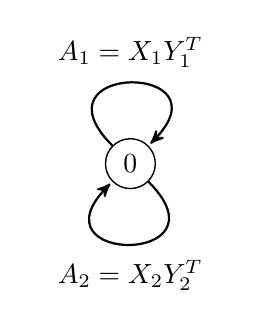
\begin{tikzpicture}
        \SetGraphUnit{3}
        \GraphInit[vstyle=Dijkstra]
        \SetUpEdge[style={->}]
        \Vertex{0}
        \Loop[labelstyle={above=2pt,fill=white},dist=1.5cm,dir=NO,label={$A_1 = X_1Y_1^T$}](0)
        \Loop[labelstyle={below=2pt,fill=white},dist=1.5cm,dir=SO,label={$A_2 = X_2Y_2^T$}](0)
      \end{tikzpicture}
      \caption{Automaton $\G$.
      We
      have $V = \{0\}$ and $E = \{(0,0,1),(0,0,2)\}$.}
      \label{fig:redu1}
    \end{subfigure}
    \begin{subfigure}{0.31\textwidth}
      \centering
      \begin{tikzpicture}
        \SetGraphUnit{3}
        \SetUpEdge[style={->}]%
        \tikzset{EdgeStyle/.style = {distance = 30}}
        \Vertex[NoLabel=false]{1}
        \EA[NoLabel=false](1){2}
        \tikzset{EdgeStyle/.append style = {bend right=60}}
        \Loop[labelstyle={above=0pt},dist=1.5cm,dir=EA,label={$A_{11}' = Y_1^TX_1$}](1)
        \Loop[labelstyle={above=0pt},dist=1.5cm,dir=EA,label={$A_{22}' = Y_2^TX_2$}](2)
        \Edge[labelstyle={above=4pt, fill opacity=0, text opacity=1},label={$A_{21}' = Y_2^\Tr X_1$}](1)(2)
        \Edge[labelstyle={below=4pt, fill opacity=0, text opacity=1},label={$A_{12}' = Y_1^\Tr X_2$}](2)(1)
      \end{tikzpicture}
      \caption{Automaton $\G'$.
      We have $V' \allowbreak= \allowbreak\{1,2\}$ and
      $E' = \{(1,1,11),\allowbreak (1,2,21),\allowbreak (2,1,12),\allowbreak (2,2,22)\}$.}
      \label{fig:redu2}
    \end{subfigure}
    \caption{Simple example of the low rank reduction.}
    \label{fig:redu}
  \end{figure}
\end{myexem}

\begin{myrem}
  The matrices $X_\sigma, Y_\sigma$ of the factorization $A_\sigma = X_\sigma Y_\sigma^T$ are not unique.
  For any invertible matrix $S \in \mathbb{R}^{r \times r}$, $A_\sigma = (X_\sigma S)(S^{-1}Y_\sigma^T)$ also gives a factorization.
  However, if $\cjsrp$ is approximated using the sum of squares algorithm of \secref{sos},
  any two factorizations will give the same approximation.
  The effect of using $X_\sigma S$ and $Y_\sigma S^{-T}$ instead of $X_\sigma$ and $Y_\sigma$ will simply be a linear change of variable of the polynomial $p_\sigma$;
  see \secref{sos}.

\end{myrem}

What is the impact of this reduction on the computational complexity and accuracy of the approximation ?
The entropy of the language of allowed switching signals is the same for the initial system and the reduced system hence the guarantee in \theoref{second} is the same for both systems.
However, the dimension of the matrices goes from the dimension of the matrices $n$ to their rank $r$
hence for low rank matrices the guarantee in \theoref{matt} is improved.

In terms of computational complexity, there can be up to $m$ \nodes{} and $m^2$ \arcs{} in the automaton of the reduced system.
Therefore, even if the size of the matrices decreases from $n$ to $r$, the number of variables and constraints increases.
This shows that the reduction only decreases the computational complexity if the rank of the matrices is \emph{sufficiently} low.


\section{Conclusions}
We have analysed the dual of the SOS Lyapunov program for switched systems
and shown how to leverage it to study the system stability.
We also generalized the whole approach to \emph{constrained switched systems},
a class of systems that has attracted increasing attention recently.

It turns out from our analysis that these two concepts are intrinsically related:
Our \theoref{fourth}, which leverages the dual of the classical JSR algorithm,
actually naturally applies to the constrained case;
Even more, \propref{Bsc} transforms an unconstrained system into a scalar constrained one for the purpose of computing a lower bound.
Finally, we show in \theoref{lowrank} that unconstrained systems with low rank matrices naturally lead to the definition of an auxiliary \emph{constrained} system.


We have introduced two techniques to generate lower bounds from the solution of the SOS dual program.
In practice, these techniques provide periodic trajectories of high asymptotic growth rate.
Since the SOS program can be solved efficiently,
does this give an efficient algorithm to generate lower bounds on the CJSR with \emph{guaranteed accuracy}?
This is not clear, because our algorithm provides firm guarantees only when the computed measures are atomic, which is not always the case.

More generally, the techniques developed in this work, based on
generating ``bad'' trajectories for a dynamical system via dual solutions%
, naturally extend to many other problems in systems theory. We are currently
exploring such possibilities.


\bibliographystyle{siamplain}
\bibliography{biblio}

\appendix
\section{Stability certificates and duality}
\begin{theorem}
  \label{theo:stabcert}
  Consider \defAGe{}.
  We have
  \[ \lim_{k \to \infty} \cjsrk \leq \gamubopt. \]
  \begin{proof}
    Consider a norm $\|\cdot\|$ of $\R^n$ and its corresponding induced matrix norm of $\R^{n \times n}$.
    For each $v \in \Nodes$, we know by compactness of the unit ball in $\R^n$, continuity and strict positivity of $f_v(x)$ that there exist $0 < \alpha_v \leq \beta_v$ such that
    \[ \alpha_v \|x\| \leq f_v(x) \leq \beta_v\|x\| \]
    for all $x \in \R^n$.
    Let $\alpha = \min_{v \in \Nodes} \alpha_v$ and $\beta = \max_{v \in \Nodes} \beta_v$.

    For a $\G$-admissible $k$-uple $(\sigma_1, \sigma_2, \ldots, \sigma_k)$,
    \[ \|A_{\sigma_k} \cdots A_{\sigma_1}\| = \sup_{x \neq 0} \frac{\|A_{\sigma_k} \cdots A_{\sigma_1}x\|}{\|x\|}. \]
    Consider a path such that the $i$th edge has label $\sigma_i$ for $i = 1, \ldots, k$
    and denote the intermediary nodes of that path as $v_0, v_1, \ldots, v_k$.
    For any $x \in \R^n$, we have
    \begin{align*}
      \|A_{\sigma_k} \cdots A_{\sigma_1}x\| %
                                            \leq \alpha_{v_k} f_{v_k}(A_{\sigma_k} \cdots A_{\sigma_1} x)%
                                            \leq \alpha_{v_k} \gamub f_{v_{k-1}}(A_{\sigma_{k-1}} \cdots A_{\sigma_1} x)%
                                            \leq \alpha_{v_k} \gamub^{k} f_{v_0}(x)
    \end{align*}
    and
    \[ \|x\| \geq \beta_{v_0} p_{v_0}(x) \]
    hence
    \[ \|A_{\sigma_k} \cdots A_{\sigma_1}\| \leq \frac{\beta_{v_0}}{\alpha_{v_k}} \gamub^k \leq \frac{\beta}{\alpha} \gamub^k. \]
    Taking the $k$th root, the limit $k \to \infty$ and using \defref{cjsr} we obtain the result.
  \end{proof}
\end{theorem}

\begin{lemma}[No duality gap]
  \label{lem:duality}
  For a fixed $\gamma$,
  \begin{description}
    \item[Weak duality] If \progref{primalinf} (resp. \progref{dualinf}) is feasible for $\gamub = \gamma$ (resp. $\gamlb = \gamma$) then \progref{dualinf} (resp. \progref{primalinf}) is infeasible for all $\gamlb < \gamma$ (resp. $\gamub > \gamma$).
    \item[Strong duality] If \progref{primalinf} (resp. dual) is infeasible for $\gamub = \gamma$ (resp. $\gamlb = \gamma$) then \progref{dualinf} (resp. \progref{primalinf}) is feasible for $\gamlb = \gamma$ (resp. $\gamub = \gamma$).
  \end{description}

  In other words, there exists a value $\gamma^*$ such that
  for every $\gamma > \gamma^*$, there exists a feasible solution to \progref{primalinf} \progref{primalinf} and
  for every $\gamma < \gamma^*$, there exists a feasible solution to \progref{dualinf} \progref{dualinf}.
  Moreover, either \progref{primalinf} program, \progref{dualinf} program or both have a feasible solution with $\gamma = \gamma^*$.
  \begin{proof}
    Consider the hyperplane
    \[ C \eqdef \Big\{\, (f_v : v \in \Nodes) \in \F^{|\Nodes|} \, \Big| \sum_{v \in V} \int_{\Sn} f_v(x) \dif x = 1 \,\Big\} \]
    and the map
    \[ \mapc_\gamma \colon \F^{|\Nodes|} \to \F^{|\Arcs|} : (f_v : v \in \Nodes) \mapsto (\gamma f_u(x) - f_v(A_\sigma x) : (u,v,\sigma) \in \Arcs). \]

    Given a fixed $\gamma$,
    \progref{primalinf} has no solution for $\gamub = \gamma$
    if and only if $\mapc_{\gamma}(\Fpp^{|\Nodes|} \cap C) \cap \Fp^{|E|} = \emptyset$.
    Since $\Fpp^{|\Nodes|} \cap C$ is compact, so is $\mapc_{\gamma}(\Fpp^{|\Nodes|} \cap C))$.
    We know that a compact set and a closed set have no intersection if and only if there exist a strict separating hyperplane separating the two sets.
    That is, a measure $\mu \in \Fbd$ such that $\la \mu, f \ra \geq 0$ for all $f \in \Fp^{|E|}$ and $\la \mu, f \ra < 0$ for all $f \in \mapc_{\gamma}(\Fpp^{|\Nodes|} \cap C)$.
    The first condition is simply $\mu \in \Fbpd$.
    For the second condition, we remark that
    \[ \mapc_{\gamma}(\Fpp^{|\Nodes|} \cap C) = \mapc_{\gamma}(\inte(\Fp^{|\Nodes|}) \cap C) = \relint\mapc_{\gamma}(\Fp^{|\Nodes|} \cap C). \]
    We have $\la \mu, f \ra < 0$ for all $f \in \relint\mapc_{\gamma}(\Fp^{|\Nodes|} \cap C)$ if and only if
    $\la \mu, f \ra \leq 0$ for all $f \in \mapc_{\gamma}(\Fp^{|\Nodes|} \cap C)$ and
    \begin{equation}
      \label{eq:affinhyp}
      \exists f \in \mapc_{\gamma}(\Fp^{|\Nodes|} \cap C) : \la \mu, f \ra \neq 0.
    \end{equation}

    Therefore, if \progref{primalinf} has no solution for $\gamub = \gamma$ then there exists
    a \emph{nonzero} measure $\mu \in (\Fbpd)^{|E|}$ such that for all $f \in C$ and $(u,v,\sigma) \in E$,
    \begin{equation}
      \label{eq:dualconsfirst}
      \sum_{v \in V} \sum_{(v,u,\sigma) \in E} \bar{\gamma} \Exp_{vu\sigma}[f_v(x)] \leq \sum_{v \in V} \sum_{(u,v,\sigma) \in E} \Exp_{uv\sigma}[f_v(A_\sigma x))]
    \end{equation}
    and \eqref{eq:affinhyp} holds.

    Note that if the inequality \eqref{eq:dualconsfirst} is respected for some $f \in C$, it is also respected for $\lambda f$ for all $\lambda > 0$.
    So we can impose that the inequality should be respected for all $f \in \Fp^{|V|} \setminus \{0\}$.

    The constraint~\eqref{eq:dualconsfirst} must be true for all $f \in \Fp^{|V|} \setminus \{0\}$ so in particular in the case where there is a node $v \in V$ such that $f_u(x) = 0$ for all $u \neq v$.
    Therefore we must have
    \[ \gamma \sum_{(v,u,\sigma) \in E} \Exp_{vu\sigma}[f_v(x)] \leq \sum_{(u,v,\sigma) \in E} \Exp_{uv\sigma}[f_v(A_\sigma x))], \quad \forall f_v \in \Fp \]
    for all $v \in V$.
    This is \eqref{eq:dualinf1} so the strong duality is proven.

    To show the weak duality, we show that if there exists a dual solution $\mu$ for $\gamlb=\gamma$ then \eqref{eq:dualinf1} and \eqref{eq:affinhyp} are satisfied for all $\gamlb < \gamma$.
    We know that \eqref{eq:dualinf1} is satisfied for $\gamma$ so the constraint \eqref{eq:dualinf1} is also satisfied for any $\gamlb < \gamma$.
    Using \eqref{eq:dualconsfirst} and \eqref{eq:dualinf3} with $f_v(x) = \|x\|$ for all $v \in \Nodes$,
    we have $\la \mu, f \ra < 0$ for all $\gamlb < \gamma$.

  \end{proof}
\end{lemma}


\section{The $p$-radius}
\label{app:pradius}
We extend the definition of the $p$-radius to the constrained case.
\begin{definition}[Constrained $p$-radius]
  The \emph{constrained $p$-radius} of
  \defAGe{}, denoted as $\cpr$,
  is
  \begin{equation*}
    \cpr =
    \lim_{k \to \infty} \left[|\Arcs_k|^{-1} \sum_{v \in V} \cprkv{k}{v}\right]^{\frac{1}{pk}}
  \end{equation*}
  where
  \begin{align*}
    \cprkv{k}{v} & =
    \sum_{s \in \Arcsout_k(v)} \|A_s\|^p.
  \end{align*}
  Thus, the CJSR can be defined as the constrained $p$-radius for $p = \infty$.
\end{definition}


\begin{myrem}
  \label{rem:path}
  Since $\G$ is assumed to be strongly connected,
  we could give the following equivalent definition
  \begin{equation}
    \label{eq:cprk2}
    \cpr = \lim_{k \to \infty}
    \left[\max_{v \in \Nodes} [\dout_k(v)]^{-1} \cprkv{k}{v}\right]^{\frac{1}{pk}}
  \end{equation}
  or the same definition with ``$\din_k(v)$'' instead of ``$\dout_k(v)$'' and ``$s \in \Arcsin_k(v)$'' instead of ``$s \in \Arcsout_k(v)$'' in the definition of $\cprkv{k}{v}$.

\end{myrem}

By the equivalence of norms, the definition of the $p$-radius does not depend on the norm used.

We can show that the $p$-radius is well defined using the following classical result, known as \emph{Fekete's Lemma} \cite{fekete1923verteilung}.
\begin{lemma}
  \label{lem:fekete}
  Let $\{a_n\} : n \geq 1$ be a sequence of real numbers such that
  \[ a_{m + n} \leq a_m + a_n. \]
  Then the limit
  \[ \lim_{n \to \infty} \frac{a_n}{n} \]
  exists and is equal to $\inf\left\{\frac{a_n}{n}\right\}$.
\end{lemma}
\begin{lemma}
  \label{lem:feketemax}
  Consider \defAGe{} and
  the sequence $(a_k)_k = \max_{v \in V} \cprkv{k}{v}$ with a submultiplicative norm.
  The sequence $\sqrt[k]{a_k}$ converges when $k \to \infty$.
  Moreover,
  \[ \lim_{k \to \infty} \sqrt[k]{a_k} = \inf \{\sqrt[k]{a_k}\}. \]

  \begin{proof}
    By submultiplicativity, for any $v \in V$, $k$ and any $k_1,k_2 \geq 0$ such that $k_1 + k_2 = k$,
    \begin{align*}
      \cprkv{k}{v}
      & = \sum_{u \in V} \sum_{s_1 \in \Arcs_{k_1}(v,u),s_2\in \Arcsout_{k_2}(u)} \|A_{s_2}A_{s_1}\|^p\\
      & \leq \sum_{u \in V} \sum_{s_1 \in \Arcs_{k_1}(v,u),s_2\in \Arcsout_{k_2}(u)} \|A_{s_2}\|^p\|A_{s_1}\|^p\\
      & = \sum_{u \in V} \cprkv{k_2}{u} \sum_{s_1 \in \Arcsin_{k_1}(u),s_1(1)=v} \|A_{s_1}\|^p\\
      & \leq a_{k_2} \sum_{u \in V} \sum_{s_1 \in \Arcsin_{k_1}(u),s_1(1)=v} \|A_{s_1}\|^p\\
      & \leq \cprkv{k_1}{v} a_{k_2}
    \end{align*}
    hence, in particular, $a_k \leq a_{k_1} a_{k_2}$ and $\log a_k \leq \log a_{k_1} + \log a_{k_2}$.
    We can conclude by \lemref{fekete}.
  \end{proof}
\end{lemma}

\begin{corollary}
  \label{coro:summax}
  The following holds
  \[ \lim_{k \to \infty} \left[\max_{v \in V} \cprkv{k}{v}\right]^{\frac{1}{k}} = \lim_{k \to \infty} \left[\sum_{v \in V} \cprkv{k}{v}\right]^{\frac{1}{k}} \]
  and, in particular, the limit on the right-hand side converges.

  \begin{proof}
    For a finite set of nonnegative numbers, their maximum is always between their average and their sum:
    \[ \frac{1}{|V|} \sum_{v \in V} \cprkv{k}{v} \leq \max_{v \in V} \cprkv{k}{v} \leq \sum_{v \in V} \cprkv{k}{v} \]
    or equivalently
    \[ \max_{v \in V} \cprkv{k}{v} \leq \sum_{v \in V} \cprkv{k}{v} \leq |V| \max_{v \in V} \cprkv{k}{v}. \]
    By \lemref{feketemax}, $\max_{v \in V} \cprkv{k}{v}$ converges for $k \to \infty$ hence $\sum_{v \in V} \cprkv{k}{v}$ converges too.
    Taking the $k$th root and the limit $k \to \infty$ gives the identity.
  \end{proof}
\end{corollary}

\begin{lemma}
  \label{lem:rhoAG}
  Consider \defAG{}.
  The following relation holds
  \[
    \cpr = \rho(A(\G))^{-\frac{1}{p}} \lim_{k \to \infty}
    \left[
      \sum_{s \in \Arcs_k} \|A_s\|^p
    \right]^{\frac{1}{pk}}.
  \]
  \begin{proof}
    By \cororef{summax},
    \[
      \lim_{k \to \infty}
      \left[
        \sum_{s \in \Arcs_k} \|A_s\|^p
      \right]^{\frac{1}{pk}}
    \]
    converges.
    It remains to show that $\lim_{k \to \infty} |\Arcs_k|^{-\frac{1}{pk}}$ converges to $\rho(A(\G))^{-\frac{1}{p}}$.

    Consider the matrix norm $\|\cdot\|_\infty$ on $\R^{n \times n}$ induced by the infinity norm on $\R^n$.
    It is well known that
    \[ \|A\|_{\infty} = \max_{1 \leq i \leq n} \sum_{j=1}^n |a_{ij}| \]
    where $a_{ij}$ is $(i,j)$ entry of $A$.
    It is also well known that the $(u,v)$ entry of $A(\G)^k$ gives                        %
    the number of paths of length $k$ starting at node $u$ and ending at node $v$ in $\G$. %
    Hence $\|A(\G)^k\|_\infty = \mdout_k(\G)$.
    By Gelfand's formula,
    \begin{equation}
      \label{eq:rhoAG}
      \rho(A(\G)) = \lim_{k \to \infty} \|A(\G)^k\|_\infty^{1/k}.
    \end{equation}
    Since $|E_k|/|V| \leq \mdout_k(\G) \leq |E_k|$,
    and $|V|^{1/k} \to 1$ as $k \to \infty$, we are done.
  \end{proof}
\end{lemma}



\begin{proof}[Proof of \lemref{incp}]
  The Lemma is a consequence of the inequality between ordinary means
  and the inequality between the $p$-norms ($p \geq 1$)
  \[ \|x\|_p = \Big(\sum_{i=1}^n |x_i|^p\Big)^{\frac{1}{p}}. \]
\end{proof}

\begin{lemma}[\cite{hardy1952inequalities}]
  For any nonnegative integers $a_1, \ldots, a_n$ and positive
  real numbers $p \leq q$,
  \[
    \left(\frac{1}{n}\sum_{i=1}^n a_i^p\right)^{\frac{1}{p}}
    \leq
    \left(\frac{1}{n}\sum_{i=1}^n a_i^q\right)^{\frac{1}{q}}
    \leq \max\{\, a_i \mid i = 1, \ldots, n\,\}.
  \]
\end{lemma}

\begin{lemma}
  For any real numbers $1 \leq p \leq q$,
  \[
    \|x\|_\infty \leq \|x\|_q \leq \|x\|_p.
  \]
\end{lemma}


Let $x^{[d]}$ denote the \emph{scaled monomial} basis.
The elements of this basis are
\[ \frac{d!}{\alpha_1!\alpha_2!\cdots\alpha_n!} x_1^{\alpha_1} \cdots x_n^{\alpha_n}. \]
for each \ktups{n} of nonnegative integers $\alpha$ such that
$\alpha_1 + \cdots + \alpha_n = d$.
For this basis, $\|x^{[d]}\|_2 = \|x\|_2^d$ where $\|\cdot\|_2$ is the Euclidean norm.


For any matrix $A \in \R^{n \times n}$, the map $x \mapsto x^{[d]}$ induces an
associated map $A^{[d]} \in \R^{N_d \times N_d}$ which is the unique
matrix that satisfies $(Ax)^{[d]} = A^{[d]}x^{[d]}$.
We also denote $\A^{[d]} \eqdef \{A_1^{[d]}, \ldots, A_m^{[d]}\}$.

Since $\|Ax\|^{[d]} = \|A\|^{[d]}\|x\|^{[d]}$, we have the following
Lemma that is known in the unconstrained case or for the contrained
case with $p=\infty$.
\begin{lemma}
  \label{lem:pp}
  Consider \defAG{}, then
  \[ \cpr[p] = \rho_1(\G,\A^{[p]})^{\frac{1}{p}} \]
  and
  \[ \cjsr = \rho(\G,\A^{[p]})^{\frac{1}{p}}. \]
\end{lemma}

We say that a cone $\Kset$ is \emph{proper} if it is closed, solid, convex and pointed.
We say that a matrix $A$ \emph{leaves a set $S$ invariant} if $AS \subseteq S$ and
we say that a set of matrices $\A$ \emph{leaves a proper cone invariant} if there
exists a proper cone $\Kset$ such that each matrix of $\A$ leaves $\Kset$ invariant.

\begin{lemma}[{\cite{blondel2005computationally,protasov1997generalized}}]
  \label{lem:unconstrainedinv}
  If a set of $m$ matrices leaves a proper cone $\Kset$ invariant, then
  \begin{align*}
    \rho_1(\A)
    & = \frac{1}{m}\lim_{k\to\infty} \left\|\sum_{s \in [m]^k}A_s\right\|^{\frac{1}{k}}\\
    & = \frac{1}{m}\rho\left(\sum_{A \in \A}A\right).
  \end{align*}
\end{lemma}


We deduce the following corollary of \lemref{pp} and
\lemref{unconstrainedinv}.
\begin{corollary}
  If $\A^{[p]}$ leaves a proper cone $\Kset$ invariant, then
  \begin{align*}
    \rho_p(\A)
    & = \frac{1}{m^{\frac{1}{p}}}\lim_{k\to\infty} \left\|\sum_{s \in [m]^k}A_s^{[p]}\right\|^{\frac{1}{pk}}\\
    & = \frac{1}{m^{\frac{1}{p}}}\rho\left(\sum_{A \in \A}A^{[p]}\right)^{\frac{1}{p}}.
  \end{align*}
\end{corollary}


We generalize it to the constrained case using the lifting procedure
introduced independantly by Kozyakin~\cite{kozyakin2014berger} and Wang~\cite{wang2014stability}.

\begin{lemma}
  \label{lem:koz}
  Consider \defAGe{}.
  The following identity holds for any $p \in [1, +\infty]$
  \[
    \sum_{s \in \Arcs_k} \|A_s\|^p =
    \sum_{s \in \Arcs^k} [\|A_s'\|']^p
  \]
  where
  \[ \A' = \{\, A'_{uv\sigma} = (e_ve_u^\Tr) \kron A_\sigma \mid (u,v,\sigma) \in E \,\}. \]
  \begin{proof}
    Consider a vector norm $\|\cdot\|$ of $\R^n$ and
    the vector norm $\|\cdot\|'$ of $\R^{n|V|}$ such that
    \[ \|e_1 \kron x_1 + \cdots + e_{|V|} \kron x_{|V|}\| = \|x_1\| + \cdots + \|x_{|V|}\|. \]
    Consider the induced matrix norms $\|\cdot\|$ and $\|\cdot\|'$.
    It is easy to see that for any nodes $u,v \in V$ and any matrix $B \in \R^{n \times n}$,
    $\|(e_ve_u^\Tr) \kron B\|' = \|B\|$.
    In particular, given a path $s \in \Arcs_k$,
    \begin{align*}
      \|A_s'\|' & = \left\|\prod_{i=1}^k(e_{s(i+1)}e_i^\Tr) \kron A_{s[i]}\right\|'\\
      & = \|(e_{s(k+1)}e_{s(1)}^\Tr) \kron A_s\|' = \|A_s\|
    \end{align*}
    and given $s \notin \Arcs_k$, $\|A_s'\| = 0$.
  \end{proof}
\end{lemma}

It is easy to see that if $\A$ leaves the proper cone $\Kset$ invariant then
the set of matrices $\A'$ of \lemref{koz} leaves the proper cone $\Kset^{|\Nodes|}$ invariant.

\begin{lemma}
  \label{lem:constrainedinv}
  Consider \defAGe{}.
  If $\A$ leaves a proper cone invariant, then
  \begin{align*}
    \cpr[1]
    & = \frac{1}{[\rho(A(G))]^{\frac{1}{p}}}\lim_{k\to\infty} \left\|\sum_{s \in \Arcs_k}(e_{s(k+1)}e_{s(1)}^\Tr) \kron A_s\right\|^{\frac{1}{k}}\\
    & = \frac{1}{[\rho(A(G))]^{\frac{1}{p}}}\rho\left(\sum_{(u,v,\sigma) \in E}(e_ve_u^\Tr) \kron A_\sigma\right).
  \end{align*}
  \begin{proof}
    Combine \lemref{rhoAG}, \lemref{koz} and \lemref{unconstrainedinv}.
  \end{proof}
\end{lemma}

\begin{theorem}
  \label{theo:norminout}
  Consider \defAG{}.
  If $\A^{[p]}$ leaves a proper cone invariant,
  the following identities hold
  \begin{align*}
    \cpr
    & = \frac{1}{[\rho(A(G))]^{\frac{1}{p}}}\lim_{k\to\infty} \left\|\sum_{s \in \Arcs_k}(e_{s(k+1)}e_{s(1)}^\Tr) \kron A_s^{[p]}\right\|^{\frac{1}{pk}}\\
    & = \frac{1}{[\rho(A(G))]^{\frac{1}{p}}}\rho\left(\sum_{(u,v,\sigma) \in E}(e_ve_u^\Tr) \kron A_\sigma^{[p]}\right)^{\frac{1}{p}}.
  \end{align*}
\end{theorem}


Theorem~\ref{theo:norminout} shows that when there is an invariant proper cone,
$\cpr$ is as easy to obtain as computing a spectral radius.

It turns out that if $p$ is even then there exists an invariant proper cone.
\begin{lemma}
  Consider \defAG{}.
  For any positive integer $d$,
  $\A^{[2d]}$ leaves an invariant proper cone.
  Moreover this cones is the cone of SOS polynomials in the
  scaled monomial basis.
  \begin{proof}
    Consider an homogeneous SOS polynomial $p(x)$ of degree $2d$ and
    its coordinates $p$ in the scaled monomial basis. That is,
    $p(x) = \la p,x^{[2d]}\ra$. For any matrix $A$, we have
    \[ \la A^{[2d]}p, x^{[2d]} \ra = \la p, (A^{[2d]})^\Tr x^{[2d]} \ra =
    \la p, (A^\Tr x)^{[2d]} \ra = p(A^\Tr x). \]
    Therefore if $p$ is the coordinate vector of an SOS polynomial
    then $A^{[2d]}p$ is also the coordinate vector of an SOS
    polynomial.
  \end{proof}
\end{lemma}


\end{document}
